%!TeX root = main.tex
%!encoding = UTF-8 Unicode

\section{Verification}

\subsection{Small-Signal}
The updated probe was validated using the methodology of~\cite{kragl_active_2025}: large-signal verification with a \SI{50}{\ohm} pulse generator, small-signal characterization with a vector network analyzer (VNA), and low-pass cross-verification against a standard passive probe to exclude unintended capacitive or inductive coupling into the active measurement path.
The VNA results for the low-pass and high-pass channels are shown in \fref{fig:VNA_LP} and \fref{fig:VNA_HP}, respectively.

\begin{figure}[ht]
	\centering
	% This file was created by matlab2tikz.
%
%The latest updates can be retrieved from
%  http://www.mathworks.com/matlabcentral/fileexchange/22022-matlab2tikz-matlab2tikz
%where you can also make suggestions and rate matlab2tikz.
%
\definecolor{mycolor1}{rgb}{0.00000,0.44700,0.74100}%
\definecolor{mycolor2}{rgb}{0.85000,0.32500,0.09800}%
\definecolor{mycolor3}{rgb}{0.92900,0.69400,0.12500}%
\definecolor{mycolor4}{rgb}{0.49400,0.18400,0.55600}%
%
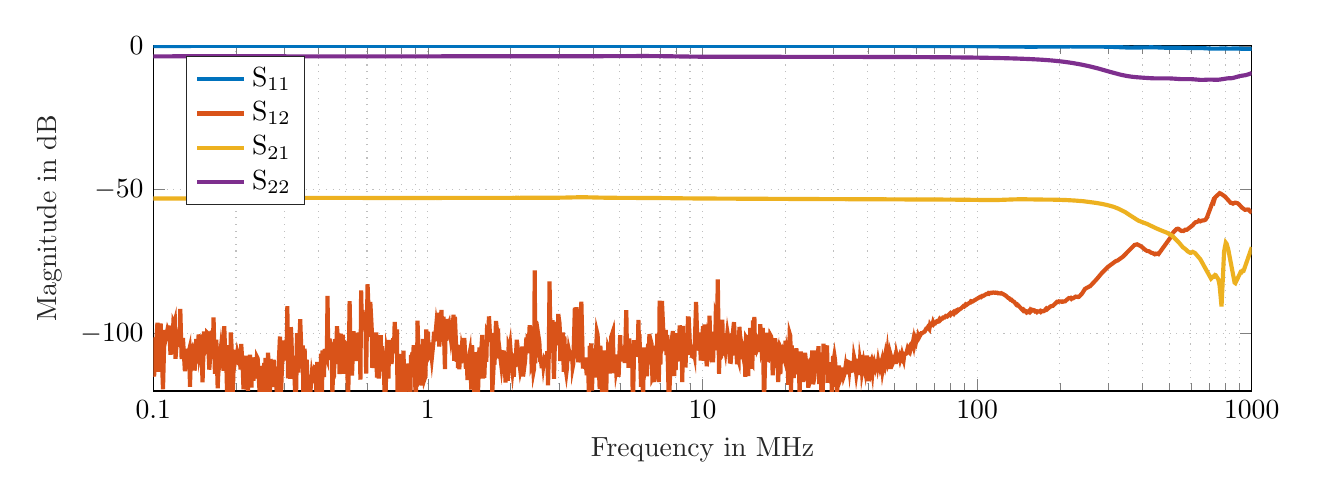
\begin{tikzpicture}

\begin{axis}[%
width=5.492in,
height=1.726in,
at={(0.921in,0.459in)},
scale only axis,
xmode=log,
xmin=0.1,
xmax=1000,
xtick={0.1,1,10,100,1000},
xticklabels={{0.1},{1},{10},{100},{1000}},
xminorticks=true,
xlabel style={font=\color{white!15!black}},
xlabel={Frequency in MHz},
ymin=-120,
ymax=0,
ylabel style={font=\color{white!15!black}},
ylabel={Magnitude in dB},
axis background/.style={fill=white},
xmajorgrids,
xminorgrids,
ymajorgrids,
grid style={dotted},
legend style={at={(0.03,0.97)}, anchor=north west, legend cell align=left, align=left, draw=white!15!black}
]
\addplot [color=mycolor1, line width=1.5pt]
  table[row sep=crcr]{%
0.1	-0.07846622336\\
0.103527468	-0.07281316743\\
0.111287897	-0.0604819558\\
0.1218703	-0.05118142218\\
0.169625017	-0.01909939471\\
0.177410572	-0.01626313434\\
0.213043601	-0.0123325037\\
0.221095909	-0.009386099722\\
0.235858474	-0.007056501781\\
0.251963091	-0.00397916227\\
0.261582765	-0.006170257478\\
0.27819181	-0.00706560105\\
0.307719002	-0.002850289133\\
0.367338544	-0.003982124183\\
0.382612797	-0.004638276902\\
0.397887049	-0.004522527786\\
0.423344138	-0.00870968907\\
0.458984061	-0.01214321664\\
0.515158441	-0.01780833359\\
0.550264191	-0.02110193266\\
0.574838217	-0.02303635007\\
0.581859367	-0.01501449397\\
0.638028568	-0.0174308464\\
0.747210132	-0.02280914783\\
0.776266149	-0.0240619522\\
0.800479497	-0.02371164862\\
0.986657469	-0.02360528924\\
1.013369958	-0.02362429898\\
1.093507426	-0.023336047\\
1.19367926	-0.02175778245\\
1.329199574	-0.01970685733\\
1.356748752	-0.01957737716\\
1.779169483	-0.01774601711\\
1.815229447	-0.01677193687\\
2.119251578	-0.01278797739\\
2.283930232	-0.01208934467\\
2.461276475	-0.01021458481\\
2.825489325	-0.007963133831\\
2.982708678	-0.008340162023\\
3.789233904	-0.006032796791\\
4.413787719	-0.004053784524\\
4.557915522	-0.004543222154\\
5.245370812	-0.003421718683\\
5.974367849	-0.004042798948\\
7.665165585	-0.004361392422\\
8.396292216	-0.004376814852\\
16.75449209	-0.01301079408\\
20.1702834	-0.01778258931\\
21.96325333	-0.01961585502\\
26.59592024	-0.02583681854\\
31.21277638	-0.02388283718\\
34.73154665	-0.022885865\\
45.88317121	-0.02382433264\\
56.2013919	-0.03600572225\\
60.9439864	-0.04418073353\\
63.10057567	-0.0466067823\\
80.78460774	-0.0709658106\\
87.28297277	-0.08771253368\\
89.66215094	-0.09608055286\\
98.58406908	-0.1228602446\\
103.3424254	-0.141600567\\
125.7477651	-0.235706467\\
129.0193635	-0.244406597\\
141.2878576	-0.2840949975\\
147.0131548	-0.2973470867\\
157.6458497	-0.3133748837\\
161.675471	-0.3101500341\\
167.3167369	-0.2959494373\\
175.2145091	-0.2691481874\\
181.9840281	-0.2481186512\\
193.2665598	-0.224600721\\
218.0881296	-0.2130461436\\
226.7613334	-0.2140140333\\
245.4318936	-0.2297653559\\
254.7671736	-0.2446945034\\
260.9906937	-0.2482738101\\
274.9936138	-0.2644505731\\
281.2171338	-0.2767142849\\
295.2200539	-0.314594602\\
313.9919762	-0.388701852\\
326.8695461	-0.460069285\\
341.8933777	-0.5385392456\\
361.2097326	-0.6270667817\\
363.3559942	-0.6296909458\\
376.2335641	-0.6051718185\\
386.9648724	-0.5690876868\\
395.549919	-0.5623482225\\
404.1349656	-0.5482955845\\
410.5737506	-0.5422699532\\
425.4457377	-0.5235677325\\
431.3651992	-0.5166038256\\
452.0833145	-0.5506225483\\
458.0027759	-0.5680771798\\
469.8416989	-0.6196249933\\
484.6403527	-0.6628363857\\
505.3584679	-0.687656716\\
517.1973909	-0.6864404092\\
523.1168524	-0.6870766127\\
531.9960446	-0.6783757616\\
543.8349676	-0.6831053609\\
570.4725443	-0.7274892639\\
576.8889099	-0.7332441373\\
585.0287378	-0.7445589042\\
593.1685657	-0.7527488083\\
617.5880494	-0.785006949\\
629.7977913	-0.7893198389\\
642.0075331	-0.7977763436\\
650.147361	-0.8082804887\\
662.3571029	-0.8134745731\\
666.4270168	-0.8169590603\\
674.5668447	-0.8420836198\\
698.9863284	-0.9300929756\\
711.1960703	-0.9631653857\\
719.3358982	-0.9825572794\\
727.4757261	-0.9876890696\\
776.3146935	-0.9514121656\\
780.3846075	-0.9535602494\\
788.5244354	-0.9470000011\\
798.8918907	-0.9410285573\\
826.9631436	-0.9749290544\\
838.1916447	-0.9698013576\\
855.0343964	-0.9460258091\\
860.648647	-0.9436667998\\
871.8771481	-0.9324516207\\
883.1056493	-0.935251179\\
894.3341504	-0.9505063803\\
928.0196538	-1.044210905\\
950.4766561	-1.061124941\\
967.3194078	-1.058622167\\
978.547909	-1.055705716\\
995.3906607	-1.065997586\\
1001.004911	-1.073095926\\
};
\addlegendentry{$\mathrm{S}_\mathrm{11}$}

\addplot [color=mycolor2, line width=1.5pt]
  table[row sep=crcr]{%
0.1	-112.8328954\\
0.100705494	-114.9842329\\
0.101410987	-101.4172326\\
0.102116481	-105.7286472\\
0.103527468	-96.24597605\\
0.104232961	-113.3339689\\
0.104938455	-100.5300715\\
0.105643948	-101.1989067\\
0.106349442	-96.4939973\\
0.108465922	-119.3674632\\
0.109876909	-98.80374902\\
0.110582403	-102.4430964\\
0.112698884	-98.48694328\\
0.113404377	-99.15804426\\
0.114109871	-97.27431293\\
0.115520858	-107.4046829\\
0.116226351	-100.2366247\\
0.116931845	-107.1522209\\
0.118342832	-96.04198044\\
0.119048325	-96.6225612\\
0.119753819	-95.70259395\\
0.120459312	-108.8167114\\
0.122575793	-98.63767665\\
0.123281287	-104.5729089\\
0.124692274	-100.5167641\\
0.125397767	-91.43354558\\
0.126808754	-108.9202416\\
0.128219741	-101.5818604\\
0.130336222	-113.0873824\\
0.131041715	-111.4814438\\
0.131747209	-105.33938\\
0.133158196	-108.2095469\\
0.135274677	-105.4934482\\
0.13598017	-118.5143202\\
0.137509601	-103.5914488\\
0.138482796	-106.619694\\
0.13945599	-105.4333694\\
0.140429185	-106.3237623\\
0.141402379	-112.9210948\\
0.143348768	-101.8896779\\
0.144321962	-110.4065857\\
0.146268351	-100.3478421\\
0.147241545	-106.5767639\\
0.14821474	-104.9026172\\
0.149187934	-100.3068082\\
0.151134323	-116.9927581\\
0.153080712	-99.25272924\\
0.154053906	-106.2848012\\
0.156000295	-104.7976404\\
0.156973489	-99.66875171\\
0.157946684	-99.91704754\\
0.159893073	-112.5703093\\
0.160866267	-108.9718097\\
0.162812656	-99.63823189\\
0.16378585	-99.54836034\\
0.164759045	-106.0811649\\
0.165732239	-94.4435988\\
0.167678628	-114.0096961\\
0.169625017	-102.1188996\\
0.171571405	-119.0802996\\
0.173517794	-107.6248561\\
0.174490989	-109.1773506\\
0.176437377	-104.707887\\
0.180330155	-112.955784\\
0.181303349	-97.49860134\\
0.183249738	-110.1750978\\
0.184222933	-107.5992622\\
0.186169321	-125.8842688\\
0.187142516	-104.6799865\\
0.18811571	-109.0997917\\
0.189088905	-104.1144604\\
0.190228728	-125.0376478\\
0.191570779	-99.6624457\\
0.19291283	-105.1243279\\
0.194254882	-124.4491932\\
0.196938984	-105.8627296\\
0.198281036	-109.8091414\\
0.199623087	-107.9122293\\
0.200965139	-108.5528656\\
0.20230719	-106.4689384\\
0.204991293	-108.5077335\\
0.206333344	-105.9350775\\
0.207675395	-112.5765818\\
0.209017447	-103.6283121\\
0.21170155	-112.1175502\\
0.213043601	-119.4335062\\
0.215727704	-111.5976296\\
0.217069755	-107.7363338\\
0.218411806	-112.7243914\\
0.219753858	-110.8545182\\
0.221095909	-119.9175259\\
0.225122063	-107.3717081\\
0.227806166	-118.7726695\\
0.229148217	-108.3554652\\
0.23183232	-116.403699\\
0.233174371	-110.1790395\\
0.234516423	-115.6598623\\
0.235858474	-108.2825623\\
0.237200526	-114.8740979\\
0.238542577	-108.1666603\\
0.239884628	-108.6285138\\
0.242568731	-116.7244955\\
0.243910782	-116.0330285\\
0.245252834	-124.1077996\\
0.246594885	-111.3093472\\
0.247936937	-118.7405038\\
0.249278988	-118.6779519\\
0.250621039	-113.7370871\\
0.251963091	-117.3532473\\
0.253305142	-110.2518996\\
0.254647193	-126.8089115\\
0.255989245	-108.4841549\\
0.257331296	-113.9442428\\
0.258673347	-109.58563\\
0.260015399	-114.8746304\\
0.261582765	-106.7168005\\
0.263428214	-111.1327106\\
0.265273664	-127.7240831\\
0.267119113	-108.9062172\\
0.270810012	-112.0843905\\
0.272655462	-116.6029107\\
0.274500911	-109.1541697\\
0.276346361	-118.6153542\\
0.27819181	-116.7564544\\
0.28003726	-112.9818942\\
0.281882709	-124.1094129\\
0.289264507	-101.0699033\\
0.291109957	-123.4888539\\
0.296646305	-102.4356459\\
0.298491755	-107.4655628\\
0.302182654	-104.8141209\\
0.305873553	-109.3359443\\
0.307719002	-90.45869933\\
0.309564452	-115.5561017\\
0.311409901	-107.390332\\
0.3151008	-115.7380408\\
0.31694625	-97.78090175\\
0.318791699	-102.3122469\\
0.320637149	-114.3707506\\
0.324328048	-107.7618168\\
0.329864396	-124.8706773\\
0.331709845	-117.97451\\
0.333555295	-99.86435405\\
0.337246194	-113.5953344\\
0.342782542	-95.06492961\\
0.346473441	-107.3422452\\
0.348318891	-108.463775\\
0.35016434	-104.1846655\\
0.35200979	-123.6116553\\
0.355700689	-105.2710058\\
0.357546138	-112.4204911\\
0.362247126	-109.1561029\\
0.364792835	-121.0929008\\
0.367338544	-116.2098495\\
0.369884252	-123.0520519\\
0.372429961	-115.9759592\\
0.37497567	-118.0069635\\
0.377521379	-114.4895708\\
0.380067088	-116.2942204\\
0.382612797	-115.6520157\\
0.387704214	-111.8855269\\
0.390249923	-112.047096\\
0.392795632	-121.1566061\\
0.395341341	-109.8614113\\
0.400432758	-123.8868573\\
0.402978467	-115.5715003\\
0.405524176	-118.5659817\\
0.408069885	-106.980466\\
0.410615594	-129.5104323\\
0.413161302	-105.9257149\\
0.41825272	-115.1245261\\
0.420798429	-105.3928398\\
0.423344138	-110.0940324\\
0.425889847	-107.6421607\\
0.428435555	-108.4326321\\
0.430981264	-86.94101807\\
0.433526973	-106.9691979\\
0.438618391	-101.7699944\\
0.443709808	-109.2454959\\
0.446255517	-104.3122229\\
0.448801226	-120.7099236\\
0.453892644	-108.6591213\\
0.456438352	-109.7866878\\
0.458984061	-101.9791526\\
0.46152977	-110.6413792\\
0.466621188	-97.44757036\\
0.471712605	-104.6086613\\
0.474258314	-102.4272372\\
0.476804023	-114.1276678\\
0.479349732	-100.696936\\
0.481895441	-100.7234403\\
0.484441149	-113.6341373\\
0.489532567	-100.3997159\\
0.492078276	-114.0472349\\
0.494623985	-105.468175\\
0.50111614	-109.2139096\\
0.504626715	-103.9079216\\
0.50813729	-104.2907881\\
0.511647866	-128.3860625\\
0.518669016	-88.73584547\\
0.522179591	-103.76244\\
0.525690166	-100.3459898\\
0.529200741	-114.6025621\\
0.536221891	-99.1862114\\
0.539732466	-109.1011481\\
0.546753616	-101.003943\\
0.550264191	-109.56135\\
0.553774767	-99.72322335\\
0.560795917	-102.8251301\\
0.564306492	-99.83083671\\
0.567817067	-116.0747093\\
0.571327642	-85.0403188\\
0.574838217	-97.17466449\\
0.578348792	-91.82044194\\
0.581859367	-98.73792579\\
0.585369942	-94.13910478\\
0.588880517	-98.89843406\\
0.592391092	-96.61737616\\
0.595901667	-113.947912\\
0.602922818	-82.90288892\\
0.613454543	-101.1156397\\
0.616965118	-89.07822109\\
0.623986268	-97.68894265\\
0.627496843	-111.961252\\
0.631007418	-110.2739545\\
0.634517993	-103.6306636\\
0.638028568	-108.7866726\\
0.645049719	-104.3960024\\
0.648560294	-99.66699246\\
0.652070869	-115.2928295\\
0.659092019	-107.3922599\\
0.662602594	-115.6365343\\
0.666113169	-109.3724861\\
0.669623744	-113.2435962\\
0.673134319	-100.5533722\\
0.676644894	-108.3263185\\
0.680155469	-104.4418836\\
0.689098098	-109.519986\\
0.698783437	-126.1190794\\
0.708468776	-106.187503\\
0.713311446	-107.6768158\\
0.718154115	-115.7053114\\
0.722996785	-102.2591842\\
0.727839454	-109.5113889\\
0.732682124	-103.8151862\\
0.737524793	-110.5904237\\
0.747210132	-101.6647646\\
0.752052802	-106.9133398\\
0.756895471	-95.98572402\\
0.76658081	-106.1443185\\
0.77142348	-98.55140102\\
0.776266149	-129.0176678\\
0.785951488	-109.0566209\\
0.795636827	-117.8557973\\
0.800479497	-107.1183956\\
0.810164836	-120.969819\\
0.815007505	-105.9548356\\
0.819850175	-119.0067582\\
0.824692844	-113.7742136\\
0.829535514	-120.572235\\
0.839220853	-110.4795735\\
0.848906192	-116.5956021\\
0.853748861	-119.028136\\
0.858591531	-114.3976076\\
0.8634342	-120.945205\\
0.86827687	-107.4187693\\
0.873119539	-111.661346\\
0.877962209	-106.477655\\
0.882804878	-108.3790836\\
0.887647548	-104.0614134\\
0.897332887	-112.0799403\\
0.902175556	-124.5193502\\
0.907018226	-115.7526847\\
0.911860895	-118.4363654\\
0.916703565	-95.55347024\\
0.926388904	-111.4129401\\
0.931231573	-110.4687555\\
0.936074243	-108.0410775\\
0.946588735	-118.0826407\\
0.95994498	-101.9114485\\
0.973301224	-115.6397862\\
0.979979347	-114.7578888\\
0.986657469	-98.62105623\\
0.993335591	-102.8960819\\
1.000013714	-99.40940356\\
1.006691836	-108.160881\\
1.013369958	-107.6191816\\
1.02004808	-103.1703346\\
1.033404325	-108.5124669\\
1.04676057	-103.3086914\\
1.053438692	-99.37100207\\
1.060116814	-102.6716684\\
1.073473059	-96.77013889\\
1.080151181	-98.50332938\\
1.086829304	-92.77572797\\
1.100185548	-104.5282699\\
1.120219915	-91.8092962\\
1.126898037	-98.61707943\\
1.13357616	-97.41356253\\
1.140254282	-94.18979973\\
1.153610527	-112.3795617\\
1.160288649	-96.11038703\\
1.166966771	-102.5548408\\
1.180323016	-94.97365787\\
1.187001138	-97.04765822\\
1.19367926	-96.42095696\\
1.213713627	-102.1084494\\
1.227069872	-98.71510117\\
1.240426117	-93.47159445\\
1.247104239	-109.4853705\\
1.253782361	-94.21262904\\
1.273816728	-109.8137606\\
1.28049485	-103.8562704\\
1.287172973	-111.9954744\\
1.293851095	-106.4282743\\
1.301650396	-112.4212324\\
1.310833455	-104.0411387\\
1.320016515	-110.3477107\\
1.329199574	-105.3610071\\
1.338382633	-106.7994947\\
1.347565693	-105.39955\\
1.356748752	-101.5401418\\
1.375114871	-112.2554258\\
1.38429793	-107.760934\\
1.393480989	-116.1747141\\
1.411847108	-108.2094835\\
1.421030167	-106.6877266\\
1.439396286	-119.5351385\\
1.448579346	-104.0653554\\
1.476128524	-120.5974419\\
1.485311583	-106.4824469\\
1.494494642	-109.8080757\\
1.512860761	-106.6042357\\
1.52204382	-120.6136249\\
1.540409939	-104.858254\\
1.549592999	-112.5031967\\
1.577142177	-100.4891485\\
1.586325236	-115.6649472\\
1.595508295	-107.6661605\\
1.604691355	-115.3971094\\
1.623057473	-102.1335531\\
1.632240533	-109.8427128\\
1.641423592	-99.30092241\\
1.650606652	-99.76461104\\
1.659789711	-99.62647515\\
1.66897277	-94.0454503\\
1.687338889	-102.3428344\\
1.696521948	-102.4101798\\
1.705705008	-99.84053136\\
1.714888067	-120.889077\\
1.742437245	-107.8368007\\
1.751620305	-108.2471058\\
1.769986423	-95.67247283\\
1.78989427	-100.0790149\\
1.802561859	-99.79235439\\
1.815229447	-108.6616235\\
1.827897036	-106.687291\\
1.853232214	-111.5216234\\
1.878567391	-106.5386361\\
1.89123498	-106.5676566\\
1.903902569	-107.6716132\\
1.916570158	-117.0881477\\
1.929237746	-110.8168211\\
1.954572924	-116.428515\\
1.967240513	-104.6060959\\
1.979908101	-105.4522075\\
1.99257569	-103.8220295\\
2.017910868	-110.8698356\\
2.030578457	-113.1103248\\
2.043246045	-110.547531\\
2.055913634	-115.0886117\\
2.068581223	-106.9380598\\
2.081248812	-111.6515449\\
2.106583989	-102.2046703\\
2.169921933	-112.8197063\\
2.182589522	-111.6414685\\
2.207924699	-104.4904523\\
2.220592288	-114.9622051\\
2.258595054	-109.6254514\\
2.283930232	-101.3685391\\
2.296597821	-105.7344264\\
2.30926541	-100.1916673\\
2.321932998	-106.9184272\\
2.347268176	-97.11177665\\
2.359935765	-105.520694\\
2.372603353	-97.51327453\\
2.385270942	-110.795962\\
2.41060612	-109.5184084\\
2.423273708	-113.4008178\\
2.435941297	-112.2799919\\
2.448608886	-78.08844622\\
2.461276475	-110.4037846\\
2.476112985	-95.66390346\\
2.493581802	-105.2664813\\
2.528519436	-101.1089127\\
2.545988253	-103.0123954\\
2.56345707	-109.3403947\\
2.580925887	-109.411927\\
2.598394704	-112.0409951\\
2.615863521	-108.1218437\\
2.633332338	-111.1352791\\
2.650801155	-109.1661194\\
2.668269972	-109.7783175\\
2.685738789	-108.8886305\\
2.703207606	-109.6146871\\
2.720676423	-106.1994213\\
2.73814524	-118.0411083\\
2.755614057	-107.146922\\
2.773082874	-81.87641345\\
2.790551691	-99.24866707\\
2.808020508	-98.16058827\\
2.825489325	-101.1433957\\
2.842958142	-95.37988791\\
2.877895776	-115.7330141\\
2.91283341	-96.02662974\\
2.930302227	-101.9412336\\
2.947771044	-96.39896525\\
2.965239861	-104.1472744\\
2.982708678	-93.23647456\\
3.017646312	-96.67212433\\
3.035115129	-109.5841357\\
3.052583946	-101.6551683\\
3.070052763	-105.0378718\\
3.087521579	-104.1179043\\
3.104990396	-99.65396324\\
3.122459213	-113.3744178\\
3.13992803	-101.0470606\\
3.174865664	-112.2723723\\
3.192334481	-113.8449357\\
3.209803298	-112.0449824\\
3.227272115	-105.3846231\\
3.244740932	-109.5453451\\
3.262209749	-105.8680044\\
3.279678566	-106.9112025\\
3.297147383	-106.8784229\\
3.3146162	-108.5550416\\
3.332085017	-108.5036134\\
3.349553834	-105.9024377\\
3.367022651	-111.6846921\\
3.384491468	-110.5715122\\
3.428914395	-91.02461264\\
3.452935696	-99.61741662\\
3.476956996	-90.85819133\\
3.500978297	-95.32504393\\
3.524999597	-110.0396065\\
3.549020898	-107.032553\\
3.573042199	-95.24921612\\
3.597063499	-95.94994435\\
3.6210848	-88.91823746\\
3.669127401	-112.1962844\\
3.693148702	-110.3875114\\
3.717170002	-110.8340815\\
3.741191303	-108.4075595\\
3.789233904	-114.5241822\\
3.813255204	-109.7643937\\
3.837276505	-112.4495337\\
3.861297806	-124.0090291\\
3.885319106	-104.3135411\\
3.909340407	-106.3031087\\
3.933361707	-103.4481362\\
3.957383008	-119.841881\\
4.005425609	-105.2515754\\
4.05346821	-115.3352893\\
4.101510811	-104.7364921\\
4.125532112	-99.42468874\\
4.149553413	-100.4347597\\
4.221617314	-119.3269786\\
4.245638615	-104.2400778\\
4.293681216	-111.0722594\\
4.317702517	-130.7411985\\
4.341723817	-106.2818879\\
4.365745118	-110.2856304\\
4.389766418	-105.8712849\\
4.413787719	-118.1025115\\
4.43780902	-109.0045388\\
4.46183032	-120.6832671\\
4.485851621	-106.9401806\\
4.509872921	-111.3803267\\
4.533894222	-104.6048765\\
4.557915522	-105.1526539\\
4.581936823	-107.3002022\\
4.605958124	-113.9737303\\
4.654000725	-101.0831341\\
4.715191149	-99.39892814\\
4.748327378	-113.7752482\\
4.781463607	-111.7537756\\
4.814599836	-107.5362292\\
4.847736065	-112.7919555\\
4.880872294	-111.0938327\\
4.914008523	-107.2875344\\
4.947144752	-115.0889259\\
5.01341721	-100.6197268\\
5.046553439	-109.7587946\\
5.079689667	-106.7080611\\
5.112825896	-108.4242704\\
5.145962125	-108.2724862\\
5.179098354	-104.5486363\\
5.212234583	-110.2700067\\
5.278507041	-91.91328568\\
5.31164327	-108.7794985\\
5.344779499	-102.3928661\\
5.377915728	-111.9108977\\
5.411051957	-101.7653982\\
5.510460644	-111.4829083\\
5.543596873	-107.6869719\\
5.576733102	-126.0130502\\
5.64300556	-102.3528397\\
5.676141789	-104.3099677\\
5.709278018	-103.8369414\\
5.742414247	-106.0271843\\
5.775550475	-102.4213658\\
5.808686704	-108.1272896\\
5.841822933	-95.24835563\\
5.874959162	-104.5425697\\
5.908095391	-103.8878916\\
5.974367849	-118.5055086\\
6.040640307	-109.185236\\
6.073776536	-124.8457594\\
6.106912765	-104.8265211\\
6.140048994	-114.0167612\\
6.173185223	-109.2625204\\
6.206321452	-111.1507006\\
6.239457681	-109.7253708\\
6.27259391	-114.8575858\\
6.338866368	-103.5953712\\
6.372002597	-110.7343993\\
6.405138826	-100.2077553\\
6.438275055	-103.1613311\\
6.477084809	-102.44293\\
6.522780223	-103.6112205\\
6.568475638	-115.4818937\\
6.614171052	-114.8567604\\
6.659866467	-116.9000249\\
6.705561881	-104.2718462\\
6.79695271	-115.9024111\\
6.842648125	-100.1127022\\
6.888343539	-102.1297712\\
6.934038953	-116.9329175\\
6.979734368	-88.61854238\\
7.025429782	-110.8011159\\
7.116820611	-88.6771949\\
7.20821144	-100.4567056\\
7.253906855	-104.0625482\\
7.299602269	-103.5553361\\
7.345297683	-98.76193279\\
7.390993098	-107.538236\\
7.436688512	-100.4686026\\
7.528079341	-121.4011801\\
7.573774756	-120.6831776\\
7.710860999	-102.9828909\\
7.802251828	-99.16997896\\
7.893642657	-114.7793909\\
7.939338071	-99.90968562\\
7.985033486	-112.7126132\\
8.0307289	-104.5907092\\
8.076424314	-108.1959443\\
8.122119729	-107.2684544\\
8.167815143	-109.6978918\\
8.259205972	-97.19684248\\
8.304901387	-99.20526768\\
8.350596801	-105.8941569\\
8.396292216	-105.6958332\\
8.44198763	-116.9093483\\
8.487683044	-97.35504252\\
8.533378459	-108.1370257\\
8.579073873	-106.8891398\\
8.624769288	-104.0267589\\
8.670464702	-111.802732\\
8.761855531	-100.1071062\\
8.807550946	-102.3391855\\
8.85324636	-94.76712607\\
8.906613499	-94.78505162\\
9.032682752	-107.3850308\\
9.095717379	-103.9544635\\
9.158752005	-107.8602857\\
9.221786632	-108.0310324\\
9.284821259	-106.0716802\\
9.347855886	-107.5196207\\
9.473925139	-89.03621532\\
9.599994392	-105.9707591\\
9.663029019	-101.5647839\\
9.726063646	-102.428168\\
9.789098272	-99.6678903\\
9.852132899	-109.4237475\\
9.915167526	-106.5900057\\
10.04123678	-97.44720646\\
10.10427141	-109.5285772\\
10.16730603	-96.90681771\\
10.23034066	-98.89253665\\
10.35640991	-111.4114598\\
10.41944454	-109.1013129\\
10.48247917	-102.5218373\\
10.54551379	-103.8315058\\
10.60854842	-93.80531673\\
10.67158305	-104.4378041\\
10.73461767	-99.42792415\\
10.7976523	-103.2363841\\
10.86068693	-102.8224896\\
10.92372155	-109.9804036\\
10.98675618	-101.9378119\\
11.11282543	-105.8220894\\
11.17586006	-93.31256765\\
11.23889469	-94.0757226\\
11.30192931	-97.90836765\\
11.36496394	-81.23160757\\
11.49103319	-114.037232\\
11.55406782	-97.45350713\\
11.61710245	-108.4817054\\
11.68013707	-108.1522227\\
11.80620633	-95.20218927\\
11.86924095	-103.4893947\\
11.93227558	-100.3471457\\
11.99531021	-107.7089334\\
12.05834483	-104.8784446\\
12.12137946	-106.1885749\\
12.32127602	-99.62942671\\
12.40820182	-101.4519556\\
12.49512763	-101.216993\\
12.58205343	-109.7856289\\
12.66897924	-109.8418038\\
12.84283085	-101.6061298\\
13.01668246	-96.06548707\\
13.19053407	-105.8955598\\
13.27745988	-105.5620442\\
13.36438568	-110.7194294\\
13.45131149	-108.4109813\\
13.53823729	-109.3664836\\
13.6251631	-97.69484953\\
13.88594051	-108.9160268\\
13.97286632	-105.8138605\\
14.05979212	-107.4277195\\
14.14671793	-104.740175\\
14.23364374	-105.2796306\\
14.32056954	-115.0651779\\
14.40749535	-101.4171507\\
14.49442115	-101.834239\\
14.58134696	-105.1713073\\
14.66827276	-114.8292217\\
14.75519857	-100.4754273\\
14.84212437	-107.5655681\\
14.92905018	-98.10947863\\
15.01597599	-112.2267686\\
15.10290179	-110.423926\\
15.1898276	-110.783122\\
15.2767534	-95.46815209\\
15.36367921	-97.95160589\\
15.45060501	-94.26330828\\
15.53753082	-107.3960367\\
15.62445662	-101.3041065\\
15.71138243	-103.7100804\\
15.79830823	-100.3352262\\
15.88523404	-105.2487518\\
16.05908565	-104.2019148\\
16.14601146	-106.3770438\\
16.23293726	-96.75887019\\
16.40678887	-105.1631018\\
16.49371468	-104.2137663\\
16.58064048	-98.05959797\\
16.75449209	-124.6407838\\
16.94293753	-105.0068784\\
17.06246886	-99.75301578\\
17.18200019	-108.9052375\\
17.30153151	-109.0684434\\
17.42106284	-104.2849932\\
17.54059417	-107.1673702\\
17.6601255	-100.5360538\\
17.77965683	-101.0459531\\
17.89918816	-104.8985293\\
18.01871949	-114.5472703\\
18.13825081	-104.1179489\\
18.25778214	-111.9498452\\
18.37731347	-101.6683242\\
18.61637613	-108.1490611\\
18.73590746	-107.0056749\\
18.85543878	-116.9179847\\
19.09450144	-104.2725346\\
19.21403277	-114.1164833\\
19.3335641	-105.2466339\\
19.45309543	-105.7623836\\
19.57262676	-110.2446118\\
19.69215808	-107.4187347\\
19.93122074	-109.2124773\\
20.05075207	-102.5408293\\
20.1702834	-111.0767886\\
20.28981473	-107.3125021\\
20.40934606	-109.032858\\
20.52887738	-117.8342234\\
20.76794004	-100.0571302\\
20.88747137	-100.8672983\\
21.0070027	-120.3724136\\
21.12653403	-104.1750417\\
21.24606536	-114.8303405\\
21.36559668	-110.1506407\\
21.48512801	-115.5113508\\
21.60465934	-112.0614973\\
21.72419067	-113.7542102\\
21.96325333	-105.1376124\\
22.08278466	-107.6131192\\
22.20231598	-114.1558136\\
22.32184731	-107.8107288\\
22.44137864	-109.5805234\\
22.56090997	-121.3885375\\
22.79997263	-106.2542194\\
23.03903528	-110.9885049\\
23.15856661	-110.7713763\\
23.29816585	-116.8385447\\
23.62794129	-106.7417115\\
23.95771673	-112.073453\\
24.12260445	-111.4419094\\
24.28749216	-118.8388964\\
24.45237988	-115.3114126\\
24.6172676	-116.0394581\\
24.78215532	-114.7324247\\
25.11193076	-105.9029666\\
25.27681848	-117.6614644\\
25.4417062	-116.1451503\\
25.77148164	-109.686473\\
25.93636936	-105.88032\\
26.10125708	-110.9624413\\
26.2661448	-110.6552167\\
26.43103252	-104.4293975\\
26.59592024	-117.6100316\\
26.92569567	-106.5696857\\
27.09058339	-120.637546\\
27.25547111	-113.0438879\\
27.42035883	-120.2902677\\
27.58524655	-103.5568823\\
27.75013427	-111.5670743\\
28.07990971	-108.2243891\\
28.40968515	-104.1409308\\
28.57457287	-117.1254892\\
29.06923603	-110.2667946\\
29.23412375	-115.8113205\\
29.39901147	-109.9491643\\
29.56389918	-120.9357506\\
29.7287869	-116.8906838\\
29.89367462	-107.807819\\
30.05856234	-109.179595\\
30.22345006	-107.6900557\\
30.38833778	-109.1565203\\
30.5532255	-113.6301547\\
30.71811322	-111.5501981\\
30.88300094	-120.9672957\\
31.3776641	-111.1565337\\
31.70743954	-116.170748\\
31.87232726	-115.6021798\\
32.03721498	-112.4527857\\
32.23033447	-114.8887266\\
32.4577174	-111.8834394\\
32.68510032	-114.8446344\\
32.91248325	-113.9777266\\
33.13986618	-111.966611\\
33.3672491	-114.148893\\
33.59463202	-109.7213942\\
34.04939788	-109.9927307\\
34.2767808	-112.3770164\\
34.50416373	-109.5480362\\
34.73154665	-113.1230917\\
34.95892958	-110.1530051\\
35.1863125	-112.907402\\
35.41369543	-112.8574467\\
35.64107835	-108.3060722\\
35.86846128	-109.5933423\\
36.32322713	-114.1278444\\
37.00537591	-108.833294\\
37.23275883	-114.4566802\\
37.46014176	-109.5105979\\
37.68752468	-111.1496335\\
37.91490761	-107.4434245\\
38.14229053	-112.9996971\\
38.59705638	-109.9892931\\
39.05182223	-112.7108356\\
39.27920516	-109.5488472\\
39.50658808	-113.6090468\\
39.73397101	-107.6057667\\
39.96135393	-116.5937875\\
40.18873686	-108.2141948\\
40.64350271	-111.2896371\\
40.87088564	-110.597192\\
41.09826856	-112.7418444\\
41.32565149	-111.7397054\\
41.55303441	-113.3503916\\
41.78041734	-110.5609721\\
42.00780026	-111.3324235\\
42.23518319	-110.2953002\\
42.46256611	-111.270447\\
42.68994904	-109.7728734\\
42.91733196	-109.8866746\\
43.14471489	-109.7364397\\
43.37209781	-111.1079371\\
43.59948074	-109.5190862\\
43.82686366	-110.6918814\\
44.05424659	-110.5359718\\
44.31980444	-111.7942082\\
44.94515115	-109.5644857\\
45.2578245	-112.8408781\\
46.19584457	-107.9641715\\
46.50851792	-110.4724544\\
46.82119127	-109.3063088\\
47.13386463	-106.6501918\\
47.44653798	-109.3717525\\
47.75921134	-108.3051294\\
48.07188469	-112.3272444\\
48.38455805	-107.3524405\\
49.32257811	-110.2982284\\
49.63525146	-109.6840358\\
50.26059817	-107.8890865\\
50.57327152	-110.5878918\\
50.88594488	-107.3591736\\
51.19861823	-108.493326\\
51.51129158	-108.3801411\\
51.82396494	-108.8139452\\
52.13663829	-108.0592178\\
52.44931165	-109.2058543\\
52.761985	-108.3924853\\
53.07465836	-108.7733708\\
53.38733171	-107.3207185\\
54.01267842	-109.0310328\\
54.32535177	-107.1263873\\
54.63802513	-107.2213749\\
55.26337183	-106.9700666\\
55.88871854	-105.0855546\\
56.51406525	-105.9419841\\
56.82673861	-105.2101485\\
57.13941196	-105.8015816\\
57.76475867	-104.0029254\\
58.07743202	-104.1839378\\
58.39010537	-102.9932821\\
58.70277873	-103.9734737\\
59.01545208	-102.1836982\\
59.32812544	-103.1947529\\
59.64079879	-102.15085\\
59.95347215	-102.8050463\\
60.2661455	-101.7542193\\
60.57881885	-101.8003909\\
60.9439864	-100.710498\\
61.37530425	-101.4660465\\
62.66925782	-99.86718114\\
63.10057567	-99.86622382\\
64.39452924	-99.35067083\\
65.25716495	-98.34386772\\
65.68848281	-98.33265741\\
66.11980066	-97.85731486\\
66.98243637	-98.51319365\\
67.41375423	-96.909182\\
67.84507208	-97.31085206\\
68.70770779	-97.00233591\\
69.13902565	-96.03421821\\
69.5703435	-96.65493267\\
70.00166136	-96.32775118\\
70.43297921	-96.42306976\\
71.29561493	-95.80776367\\
71.72693278	-95.93778464\\
72.15825064	-95.89015631\\
73.02088635	-95.01342707\\
73.4522042	-95.33557685\\
74.31483991	-94.81860545\\
74.74615777	-94.80591086\\
75.17747562	-94.45134119\\
75.60879348	-94.47018088\\
76.04011133	-94.46172245\\
76.90274704	-93.92875398\\
77.76538276	-94.09141703\\
79.49065418	-93.16136459\\
79.92197203	-93.4256532\\
80.35328989	-93.00590027\\
80.78460774	-93.16433699\\
82.07856131	-92.54652151\\
82.50987916	-92.96634008\\
83.37251487	-92.31772006\\
83.80383273	-92.14437329\\
84.30900005	-92.45031358\\
84.90379459	-92.18875798\\
85.49858914	-91.68542373\\
86.09338368	-91.7107112\\
87.28297277	-91.32986949\\
89.0673564	-90.49667955\\
89.66215094	-90.62434503\\
90.85174002	-89.89724894\\
91.44653457	-90.08416905\\
92.63612365	-89.67333454\\
93.82571274	-89.33222408\\
94.42050728	-89.27467261\\
95.01530183	-88.76877803\\
96.20489091	-88.89832236\\
99.17886362	-88.1161245\\
102.7476309	-87.24989508\\
103.3424254	-87.36165932\\
104.5320145	-86.93673651\\
105.1268091	-86.98643956\\
108.1007818	-86.28216359\\
108.6955763	-86.31805849\\
109.2903709	-86.26190433\\
109.8851654	-86.00161294\\
110.4799599	-86.13574839\\
111.0747545	-85.88338044\\
111.669549	-85.88798403\\
112.2643436	-85.83843044\\
112.8591381	-85.9253773\\
114.6435217	-85.73988353\\
115.9329699	-85.86020632\\
116.7508695	-85.77783417\\
117.5687691	-85.85942205\\
118.3866687	-85.81955355\\
119.2045683	-86.03686317\\
120.0224679	-86.02864662\\
121.6582671	-86.09288143\\
122.4761667	-85.97250921\\
126.5656647	-86.70087204\\
129.8372631	-87.63566242\\
130.6551627	-87.7276488\\
132.2909619	-88.25630436\\
133.1088616	-88.23274259\\
134.7446608	-88.75375218\\
136.38046	-88.99237082\\
138.8341588	-89.95734768\\
139.6520584	-89.87752921\\
140.469958	-90.28471585\\
141.2878576	-90.26752296\\
147.0131548	-92.02900625\\
147.8310544	-91.75252849\\
151.1026529	-92.66618656\\
151.9205525	-92.43089831\\
152.7384521	-92.55930623\\
154.3742513	-92.16131619\\
155.1921509	-92.39974511\\
156.0100505	-91.96679954\\
156.8279501	-92.29178571\\
158.4637493	-91.81927035\\
159.4189647	-91.98891975\\
160.5472178	-91.8778117\\
161.675471	-91.97708608\\
162.8037242	-92.37012184\\
163.9319773	-92.31866558\\
165.0602305	-92.58538577\\
166.1884837	-92.30970293\\
168.44499	-92.3970488\\
169.5732432	-92.18448067\\
170.7014964	-92.48561693\\
171.8297495	-92.21217642\\
172.9580027	-92.30564673\\
175.2145091	-92.20678079\\
178.5992686	-91.34508004\\
179.7275217	-91.63073371\\
185.3687876	-90.55553275\\
187.6252939	-90.43016044\\
188.7535471	-90.39441074\\
194.394813	-89.23130036\\
195.5230661	-88.97613386\\
197.7795725	-89.03239206\\
198.9078257	-88.83711203\\
201.164332	-88.90831931\\
202.2925852	-88.89551425\\
203.4208383	-88.97509777\\
204.5490915	-88.86792718\\
205.6773447	-88.94746698\\
207.933851	-88.82223828\\
209.0621042	-88.82667581\\
214.7033701	-87.85247503\\
215.8316232	-87.70446444\\
218.0881296	-87.78076823\\
219.2163827	-87.65420322\\
220.5378134	-87.96046884\\
222.0936934	-87.72195393\\
223.6495734	-87.77271494\\
228.3172134	-87.18971974\\
229.8730935	-87.25044379\\
231.4289735	-87.22413119\\
232.9848535	-87.3125446\\
234.5407335	-87.29374204\\
240.7642535	-86.19301635\\
246.9877736	-84.51788356\\
256.3230536	-83.64653012\\
257.8789337	-83.57316163\\
271.8818538	-81.23902688\\
284.3288938	-79.03119291\\
299.8876939	-76.81010879\\
320.4307612	-74.80422499\\
324.7232845	-74.64288847\\
339.7471161	-73.287737\\
374.0873025	-69.24233271\\
382.6723491	-69.0089267\\
395.549919	-69.7026498\\
410.5737506	-71.00649611\\
417.0125355	-71.36699479\\
419.5262762	-71.38104869\\
422.486007	-71.42975029\\
431.3651992	-71.98042233\\
434.32493	-71.98555918\\
443.2041222	-72.45557565\\
446.163853	-72.27640874\\
449.1235837	-72.3706036\\
455.0430452	-72.17586713\\
458.0027759	-72.35246441\\
505.3584679	-66.7251099\\
514.2376601	-65.18209915\\
531.9960446	-63.71275688\\
537.9155061	-63.57629647\\
540.8752369	-63.62646448\\
552.7141599	-64.29214146\\
555.6738906	-64.3585455\\
558.6336214	-64.31734123\\
564.5530828	-64.3770871\\
573.4322751	-63.89772425\\
576.8889099	-63.89123612\\
580.9588239	-63.93172929\\
609.4482215	-62.39827975\\
617.5880494	-61.72537321\\
625.7278773	-61.28607718\\
629.7977913	-61.26160232\\
637.9376192	-61.06435803\\
642.0075331	-60.75823152\\
650.147361	-61.00487982\\
658.2871889	-60.76015235\\
662.3571029	-60.7352465\\
670.4969308	-60.65890765\\
678.6367587	-60.44924958\\
686.7765866	-59.69696411\\
723.4058122	-53.96259901\\
727.4757261	-54.24694925\\
735.615554	-52.69901013\\
764.1049517	-51.22567239\\
772.2447796	-51.40823197\\
798.8918907	-52.38358959\\
838.1916447	-54.57730545\\
843.8058953	-54.60497511\\
855.0343964	-54.85885942\\
866.2628976	-54.56822898\\
871.8771481	-54.51865897\\
888.7198998	-54.73562791\\
899.948401	-55.17741057\\
922.4054033	-56.30392915\\
944.8624056	-56.9880244\\
950.4766561	-56.97633676\\
961.7051573	-56.9147045\\
967.3194078	-56.93826005\\
972.9336584	-56.9309602\\
1001.004911	-58.08216826\\
};
\addlegendentry{$\mathrm{S}_\mathrm{12}$}

\addplot [color=mycolor3, line width=1.5pt]
  table[row sep=crcr]{%
0.1	-53.10200347\\
0.100705494	-53.10656881\\
0.102116481	-53.09606496\\
0.103527468	-53.10380832\\
0.104938455	-53.08514251\\
0.105643948	-53.09556324\\
0.106349442	-53.08829385\\
0.108465922	-53.0921925\\
0.109171416	-53.08126028\\
0.109876909	-53.08741987\\
0.110582403	-53.08041209\\
0.11199339	-53.08723736\\
0.112698884	-53.08121118\\
0.114109871	-53.08390229\\
0.114815364	-53.07927998\\
0.116931845	-53.08835442\\
0.117637338	-53.08346139\\
0.119753819	-53.08632389\\
0.121164806	-53.08533673\\
0.1218703	-53.08727734\\
0.122575793	-53.09992046\\
0.123281287	-53.08978805\\
0.12398678	-53.0936097\\
0.125397767	-53.08845724\\
0.126808754	-53.09104687\\
0.128219741	-53.08200481\\
0.129630728	-53.08588104\\
0.131041715	-53.0687493\\
0.132452703	-53.08091323\\
0.13386369	-53.07191618\\
0.136685664	-53.06786472\\
0.137509601	-53.06624406\\
0.138482796	-53.05729717\\
0.141402379	-53.06560548\\
0.143348768	-53.05689994\\
0.144321962	-53.05074197\\
0.145295157	-53.05486521\\
0.146268351	-53.05196501\\
0.147241545	-53.05965045\\
0.14821474	-53.05223634\\
0.150161129	-53.05504206\\
0.151134323	-53.05350356\\
0.153080712	-53.04172519\\
0.154053906	-53.04513341\\
0.156973489	-53.0389744\\
0.157946684	-53.0338345\\
0.158919878	-53.03929711\\
0.159893073	-53.03460047\\
0.161839461	-53.03602848\\
0.16378585	-53.03136464\\
0.164759045	-53.02938683\\
0.167678628	-53.03179126\\
0.171571405	-53.027359\\
0.173517794	-53.02581968\\
0.174490989	-53.02180024\\
0.175464183	-53.02580941\\
0.177410572	-53.01981153\\
0.178383766	-53.02368752\\
0.181303349	-53.0127992\\
0.182276544	-53.0174028\\
0.183249738	-53.00897958\\
0.184222933	-53.01236412\\
0.186169321	-52.99767229\\
0.187142516	-53.00651066\\
0.189088905	-53.00092047\\
0.190228728	-53.00457541\\
0.191570779	-53.00392771\\
0.194254882	-52.99216792\\
0.195596933	-52.99775416\\
0.198281036	-52.9945699\\
0.200965139	-52.98410091\\
0.20230719	-52.98734156\\
0.204991293	-52.97516203\\
0.207675395	-52.97973002\\
0.209017447	-52.97275986\\
0.210359498	-52.97668633\\
0.213043601	-52.97008368\\
0.219753858	-52.96042155\\
0.221095909	-52.96433483\\
0.22243796	-52.95832957\\
0.223780012	-52.96194007\\
0.226464115	-52.95581809\\
0.227806166	-52.95065066\\
0.229148217	-52.95419436\\
0.230490269	-52.9478464\\
0.23183232	-52.94914499\\
0.233174371	-52.95413985\\
0.235858474	-52.94504624\\
0.238542577	-52.93988707\\
0.24122668	-52.93978063\\
0.245252834	-52.93253601\\
0.249278988	-52.92705213\\
0.251963091	-52.93023996\\
0.257331296	-52.91927645\\
0.258673347	-52.92178504\\
0.260015399	-52.91517917\\
0.261582765	-52.92343804\\
0.267119113	-52.9141309\\
0.270810012	-52.91938585\\
0.276346361	-52.91436487\\
0.27819181	-52.91451963\\
0.28003726	-52.9072099\\
0.281882709	-52.90868656\\
0.285573608	-52.90346158\\
0.289264507	-52.90371086\\
0.291109957	-52.89764918\\
0.296646305	-52.89893929\\
0.298491755	-52.89718555\\
0.302182654	-52.88918735\\
0.305873553	-52.89725063\\
0.307719002	-52.89049567\\
0.309564452	-52.89355995\\
0.313255351	-52.89313924\\
0.318791699	-52.89109063\\
0.320637149	-52.88496454\\
0.326173497	-52.89151464\\
0.329864396	-52.88500878\\
0.333555295	-52.88516699\\
0.337246194	-52.88150084\\
0.339091643	-52.88332224\\
0.342782542	-52.88070899\\
0.344627992	-52.87895275\\
0.346473441	-52.88485597\\
0.353855239	-52.87976149\\
0.355700689	-52.88273249\\
0.359701417	-52.87315638\\
0.362247126	-52.87590782\\
0.364792835	-52.87336679\\
0.369884252	-52.87784217\\
0.372429961	-52.87813022\\
0.37497567	-52.87211928\\
0.377521379	-52.874888\\
0.380067088	-52.87242708\\
0.382612797	-52.87593324\\
0.387704214	-52.87354398\\
0.390249923	-52.87508466\\
0.395341341	-52.87163583\\
0.405524176	-52.87410014\\
0.410615594	-52.8707129\\
0.413161302	-52.86767499\\
0.415707011	-52.87040414\\
0.425889847	-52.86595537\\
0.428435555	-52.86926642\\
0.433526973	-52.86142487\\
0.436072682	-52.86776157\\
0.441164099	-52.85926962\\
0.446255517	-52.86539484\\
0.456438352	-52.8581742\\
0.46152977	-52.86486569\\
0.469166896	-52.8645377\\
0.474258314	-52.86148188\\
0.479349732	-52.86556037\\
0.484441149	-52.86292766\\
0.486986858	-52.86541332\\
0.489532567	-52.86364955\\
0.497605565	-52.86829639\\
0.50111614	-52.86573118\\
0.504626715	-52.8714507\\
0.50813729	-52.86684653\\
0.511647866	-52.86924897\\
0.515158441	-52.86800679\\
0.525690166	-52.87171737\\
0.532711316	-52.86884934\\
0.536221891	-52.86441735\\
0.539732466	-52.86655083\\
0.546753616	-52.86315848\\
0.550264191	-52.86687476\\
0.553774767	-52.86322685\\
0.557285342	-52.86853875\\
0.560795917	-52.86294912\\
0.564306492	-52.86485119\\
0.567817067	-52.86059797\\
0.574838217	-52.86516796\\
0.581859367	-52.89242856\\
0.585369942	-52.88178345\\
0.588880517	-52.88904125\\
0.592391092	-52.8851466\\
0.599412243	-52.88549287\\
0.606433393	-52.88315079\\
0.613454543	-52.88740417\\
0.620475693	-52.88630293\\
0.623986268	-52.89096983\\
0.627496843	-52.88564915\\
0.638028568	-52.88977818\\
0.648560294	-52.88659626\\
0.655581444	-52.88878232\\
0.676644894	-52.88586415\\
0.680155469	-52.89118023\\
0.693940768	-52.88924751\\
0.698783437	-52.89247153\\
0.703626107	-52.88440902\\
0.713311446	-52.892302\\
0.722996785	-52.89079816\\
0.737524793	-52.8914021\\
0.742367463	-52.89377162\\
0.752052802	-52.88827149\\
0.756895471	-52.89420067\\
0.76658081	-52.8905167\\
0.776266149	-52.89257086\\
0.785951488	-52.88465072\\
0.795636827	-52.89073248\\
0.824692844	-52.88852114\\
0.834378183	-52.89162025\\
0.848906192	-52.88566814\\
0.8634342	-52.89133129\\
0.882804878	-52.88333872\\
0.897332887	-52.88947992\\
0.907018226	-52.88609284\\
0.911860895	-52.89144765\\
0.916703565	-52.88342024\\
0.926388904	-52.8899495\\
0.931231573	-52.8854987\\
0.940916912	-52.88964872\\
0.953266857	-52.88463233\\
0.979979347	-52.88883196\\
0.993335591	-52.88490035\\
1.000013714	-52.88172921\\
1.02004808	-52.88553062\\
1.026726203	-52.88619317\\
1.04676057	-52.87886926\\
1.053438692	-52.88545159\\
1.066794937	-52.87717133\\
1.080151181	-52.88216275\\
1.086829304	-52.87819091\\
1.100185548	-52.88183413\\
1.120219915	-52.8783912\\
1.173644894	-52.8758069\\
1.187001138	-52.87370083\\
1.19367926	-52.87618146\\
1.200357383	-52.87068774\\
1.207035505	-52.87680727\\
1.213713627	-52.87067977\\
1.227069872	-52.87260434\\
1.233747994	-52.87088712\\
1.240426117	-52.87460324\\
1.247104239	-52.86897798\\
1.253782361	-52.87512511\\
1.273816728	-52.86955121\\
1.287172973	-52.87103355\\
1.310833455	-52.86692822\\
1.320016515	-52.87070181\\
1.338382633	-52.86579891\\
1.356748752	-52.86348098\\
1.365931811	-52.86645591\\
1.375114871	-52.86219519\\
1.38429793	-52.86733494\\
1.421030167	-52.86169072\\
1.448579346	-52.86058407\\
1.466945464	-52.86201795\\
1.476128524	-52.85760646\\
1.485311583	-52.86136189\\
1.494494642	-52.85917625\\
1.503677702	-52.86118369\\
1.53122688	-52.85777117\\
1.549592999	-52.85996408\\
1.567959117	-52.85576615\\
1.586325236	-52.85914162\\
1.604691355	-52.85385931\\
1.613874414	-52.85989801\\
1.66897277	-52.85329775\\
1.687338889	-52.85751079\\
1.696521948	-52.85450683\\
1.705705008	-52.85798892\\
1.733254186	-52.85485565\\
1.751620305	-52.85158892\\
1.769986423	-52.85478326\\
1.802561859	-52.85429034\\
1.815229447	-52.85110836\\
1.853232214	-52.8541483\\
1.903902569	-52.85000369\\
1.929237746	-52.8513634\\
1.954572924	-52.84522969\\
1.979908101	-52.85038434\\
2.043246045	-52.84351914\\
2.068581223	-52.84735769\\
2.0939164	-52.83951936\\
2.119251578	-52.84604395\\
2.131919167	-52.83991242\\
2.157254344	-52.84537085\\
2.195257111	-52.84049332\\
2.220592288	-52.84332871\\
2.245927466	-52.84252471\\
2.271262643	-52.83866675\\
2.334600587	-52.83856554\\
2.359935765	-52.8376827\\
2.385270942	-52.84138125\\
2.397938531	-52.83307223\\
2.41060612	-52.83780078\\
2.423273708	-52.8355423\\
2.435941297	-52.83953688\\
2.461276475	-52.83502482\\
2.476112985	-52.83711524\\
2.511050619	-52.83552485\\
2.528519436	-52.83510249\\
2.56345707	-52.83123968\\
2.598394704	-52.83212416\\
2.633332338	-52.82638252\\
2.650801155	-52.82780659\\
2.703207606	-52.82031044\\
2.755614057	-52.8233378\\
2.790551691	-52.81437205\\
2.808020508	-52.81897395\\
2.842958142	-52.81398717\\
2.895364593	-52.80266443\\
2.91283341	-52.80773422\\
2.965239861	-52.79612272\\
3.000177495	-52.7962392\\
3.087521579	-52.77677288\\
3.104990396	-52.77397214\\
3.13992803	-52.76301492\\
3.157396847	-52.7615114\\
3.227272115	-52.74218479\\
3.573042199	-52.64077526\\
3.6210848	-52.64233326\\
3.6451061	-52.64070809\\
3.765212603	-52.6566847\\
3.933361707	-52.69252678\\
4.005425609	-52.71435707\\
4.05346821	-52.72743631\\
4.077489511	-52.72944175\\
4.149553413	-52.75110126\\
4.221617314	-52.76632776\\
4.389766418	-52.79612705\\
4.485851621	-52.81069429\\
4.605958124	-52.82374298\\
4.629979424	-52.82723431\\
4.654000725	-52.82524124\\
4.715191149	-52.83511709\\
4.947144752	-52.84782055\\
4.980280981	-52.85113166\\
5.01341721	-52.8490346\\
5.079689667	-52.85468993\\
5.179098354	-52.86059863\\
5.212234583	-52.86510616\\
5.31164327	-52.86213486\\
5.377915728	-52.86712601\\
5.411051957	-52.86400306\\
5.477324415	-52.87162255\\
5.543596873	-52.86878562\\
5.576733102	-52.8740282\\
5.64300556	-52.87384521\\
5.709278018	-52.87803925\\
5.974367849	-52.87982544\\
6.007504078	-52.88793236\\
6.040640307	-52.88485566\\
6.140048994	-52.88815788\\
6.27259391	-52.89145527\\
6.338866368	-52.8945357\\
6.372002597	-52.89155239\\
6.405138826	-52.8965463\\
6.438275055	-52.89401157\\
6.659866467	-52.9083143\\
6.751257296	-52.91145058\\
6.79695271	-52.90973555\\
6.888343539	-52.91874112\\
7.345297683	-52.94482844\\
7.573774756	-52.95823514\\
8.122119729	-53.00019714\\
8.167815143	-52.99786146\\
8.396292216	-53.01513605\\
8.761855531	-53.0307137\\
8.85324636	-53.03826674\\
9.473925139	-53.06212331\\
9.536959766	-53.05999221\\
9.663029019	-53.06708385\\
9.978202153	-53.07753112\\
10.04123678	-53.0754648\\
10.29337529	-53.08613585\\
10.35640991	-53.08398715\\
10.48247917	-53.08695711\\
10.73461767	-53.09450769\\
10.92372155	-53.09923428\\
10.98675618	-53.09630461\\
11.04979081	-53.09839388\\
11.17586006	-53.10612357\\
11.23889469	-53.10432151\\
11.61710245	-53.11253781\\
11.80620633	-53.11340414\\
12.18441409	-53.12233372\\
12.24744871	-53.11965425\\
12.32127602	-53.12396593\\
12.49512763	-53.12415012\\
12.66897924	-53.127828\\
12.84283085	-53.13212591\\
13.01668246	-53.13379965\\
13.10360827	-53.13327246\\
13.27745988	-53.14027379\\
13.36438568	-53.13870073\\
13.45131149	-53.14125599\\
13.53823729	-53.13876066\\
13.7120889	-53.14788764\\
13.79901471	-53.14396519\\
13.88594051	-53.15031977\\
13.97286632	-53.14618067\\
14.40749535	-53.15244963\\
14.49442115	-53.15961734\\
14.66827276	-53.15363923\\
14.92905018	-53.1635044\\
15.1898276	-53.16500325\\
18.13825081	-53.20032843\\
18.4968448	-53.20773272\\
18.61637613	-53.20213019\\
18.85543878	-53.20738727\\
20.05075207	-53.21786748\\
20.1702834	-53.22525034\\
20.40934606	-53.22210208\\
20.76794004	-53.23138618\\
21.0070027	-53.229919\\
21.12653403	-53.22791991\\
21.24606535	-53.23718352\\
21.36559668	-53.23159895\\
21.72419067	-53.23722577\\
21.96325333	-53.23648485\\
22.20231598	-53.24181828\\
22.79997263	-53.24856483\\
22.91950396	-53.24473593\\
23.29816585	-53.25225149\\
25.27681848	-53.27067588\\
25.4417062	-53.26773973\\
25.77148164	-53.27497925\\
25.93636936	-53.27391579\\
26.10125708	-53.27898122\\
26.2661448	-53.27407391\\
26.92569567	-53.28174421\\
28.24479743	-53.28958373\\
28.40968515	-53.28637315\\
28.73946059	-53.29200007\\
29.56389918	-53.29234901\\
30.05856234	-53.29654998\\
30.71811322	-53.3001663\\
30.88300094	-53.30510268\\
31.04788866	-53.30115582\\
31.3776641	-53.30460163\\
32.03721498	-53.30447011\\
32.23033447	-53.30238126\\
32.68510032	-53.31052653\\
33.13986618	-53.31228511\\
33.3672491	-53.31584338\\
33.59463203	-53.31019139\\
33.82201495	-53.31432399\\
34.04939788	-53.31352731\\
34.73154665	-53.3183584\\
34.95892958	-53.31572503\\
35.41369543	-53.32003889\\
36.0958442	-53.32398889\\
36.32322713	-53.32141552\\
36.77799298	-53.32626054\\
37.00537591	-53.32373365\\
37.68752468	-53.33012183\\
38.14229053	-53.33066259\\
38.59705638	-53.33472949\\
39.05182223	-53.33514455\\
39.27920516	-53.33098189\\
39.50658808	-53.33754762\\
39.73397101	-53.33579391\\
40.64350271	-53.341342\\
42.91733196	-53.34872799\\
43.59948074	-53.35465083\\
43.82686366	-53.35052986\\
44.31980444	-53.35646637\\
44.94515115	-53.3585429\\
45.2578245	-53.35797149\\
46.19584457	-53.36625368\\
46.50851792	-53.36137742\\
46.82119127	-53.36814476\\
47.13386463	-53.36738258\\
47.75921134	-53.37117916\\
48.07188469	-53.36993132\\
48.38455805	-53.37463629\\
48.6972314	-53.37244928\\
49.63525146	-53.37802645\\
49.94792482	-53.37690312\\
50.57327152	-53.38497588\\
50.88594488	-53.38278528\\
55.88871854	-53.40623399\\
56.51406525	-53.40504597\\
57.13941196	-53.40797095\\
58.39010537	-53.41387757\\
58.70277873	-53.41054408\\
59.01545208	-53.41711859\\
59.64079879	-53.41362276\\
60.2661455	-53.41695213\\
60.9439864	-53.41968356\\
61.37530425	-53.41741948\\
61.80662211	-53.42033134\\
62.23793996	-53.4192236\\
62.66925782	-53.42298448\\
63.53189353	-53.42235986\\
65.25716495	-53.42732305\\
65.68848281	-53.42453586\\
66.11980066	-53.42794043\\
66.55111852	-53.42597587\\
67.41375423	-53.43407726\\
70.86429707	-53.44133497\\
71.72693278	-53.44377634\\
72.58956849	-53.44536386\\
74.31483991	-53.45194331\\
74.74615777	-53.44958962\\
76.90274704	-53.46068209\\
77.76538275	-53.45842069\\
79.05933632	-53.46494838\\
79.92197203	-53.47196025\\
80.35328989	-53.46869926\\
82.07856131	-53.47724842\\
83.80383273	-53.48925927\\
92.63612365	-53.52942497\\
93.2309182	-53.53742833\\
94.42050728	-53.53861802\\
97.39448	-53.55438383\\
97.98927454	-53.55571062\\
99.77365817	-53.56835191\\
102.1528363	-53.57829804\\
103.93722	-53.59412478\\
104.5320145	-53.59557099\\
105.1268091	-53.60412851\\
106.9111927	-53.60731452\\
109.2903709	-53.6205172\\
109.8851654	-53.61779174\\
110.4799599	-53.62233905\\
112.8591381	-53.62134436\\
115.9329699	-53.61439839\\
118.3866687	-53.59703572\\
119.2045683	-53.59440984\\
131.4730623	-53.44086825\\
136.38046	-53.38678471\\
140.469958	-53.35904435\\
142.1057572	-53.35564653\\
143.7415564	-53.35701403\\
147.0131548	-53.35312663\\
150.2847533	-53.35733735\\
156.8279501	-53.38496011\\
158.4637493	-53.39146818\\
160.5472178	-53.39967587\\
175.2145091	-53.45903588\\
176.3427622	-53.45713606\\
178.5992686	-53.46582497\\
179.7275217	-53.46425854\\
186.4970408	-53.4855917\\
188.7535471	-53.48438718\\
191.0100535	-53.49447226\\
193.2665598	-53.50505893\\
210.1903574	-53.61067275\\
226.7613334	-53.78754364\\
243.8760136	-54.0286154\\
271.8818538	-54.6226841\\
284.3288938	-54.95361268\\
296.7759339	-55.32494303\\
313.9919762	-55.96417114\\
326.8695461	-56.60940741\\
346.185901	-57.80299282\\
356.9172093	-58.6517992\\
386.9648724	-60.79852233\\
417.0125355	-61.97134353\\
449.1235837	-63.46728277\\
452.0833145	-63.54928031\\
460.9625067	-63.92535216\\
490.5598142	-64.95549314\\
505.3584679	-65.64526377\\
511.2779294	-65.90441481\\
540.8752369	-68.20028315\\
561.5933521	-70.03574936\\
573.4322751	-70.66957752\\
585.0287378	-71.46097819\\
597.2384797	-71.96643263\\
601.3083936	-71.95080743\\
609.4482215	-71.61931328\\
621.6579634	-72.02422477\\
650.147361	-74.22338193\\
711.1960703	-80.94179353\\
723.4058122	-80.22696513\\
727.4757261	-80.26472279\\
735.615554	-79.6650723\\
739.685468	-79.75803506\\
747.8252959	-80.50219103\\
755.9651238	-81.19952521\\
764.1049517	-83.41168926\\
776.3146935	-90.64259246\\
793.2776401	-71.51674104\\
804.5061413	-68.44467437\\
810.1203919	-68.83821567\\
821.348893	-70.78406304\\
866.2628976	-82.30501443\\
871.8771481	-82.50116083\\
911.1769021	-78.65748995\\
916.7911527	-78.74383129\\
922.4054033	-78.31366499\\
928.0196538	-78.40262887\\
933.6339044	-78.28613113\\
1001.004911	-69.99797315\\
};
\addlegendentry{$\mathrm{S}_\mathrm{21}$}

\addplot [color=mycolor4, line width=1.5pt]
  table[row sep=crcr]{%
0.1	-3.681131481\\
0.104232961	-3.675637459\\
0.106349442	-3.67295822\\
0.115520858	-3.658885458\\
0.119048325	-3.651982982\\
0.119753819	-3.653260582\\
0.123281287	-3.647216302\\
0.129630728	-3.644341078\\
0.144321962	-3.639493345\\
0.146268351	-3.636619026\\
0.153080712	-3.63157445\\
0.156973489	-3.632077107\\
0.171571405	-3.63245694\\
0.209017447	-3.64611762\\
0.218411806	-3.642026548\\
0.23183232	-3.642532213\\
0.237200526	-3.644876025\\
0.270810012	-3.651433902\\
0.367338544	-3.661161534\\
0.413161302	-3.668102612\\
0.497605565	-3.671476682\\
0.574838217	-3.670727196\\
0.581859367	-3.661175242\\
0.609943968	-3.660616882\\
0.680155469	-3.663805297\\
0.752052802	-3.662699718\\
0.815007505	-3.659299616\\
0.902175556	-3.659860625\\
1.439396286	-3.649764368\\
1.549592999	-3.650034356\\
1.641423592	-3.64898763\\
3.262209749	-3.621953964\\
3.693148702	-3.613522891\\
3.933361707	-3.611985741\\
4.389766418	-3.60184672\\
5.344779499	-3.576038584\\
5.841822933	-3.566592078\\
6.338866368	-3.567116851\\
6.659866467	-3.575266908\\
6.842648125	-3.582913172\\
7.162516026	-3.601803911\\
7.528079341	-3.630087136\\
8.0307289	-3.674107392\\
8.624769288	-3.722588942\\
9.032682752	-3.749208903\\
9.663029019	-3.778224636\\
10.16730603	-3.792980719\\
11.86924095	-3.814199647\\
13.6251631	-3.819781859\\
15.97215984	-3.822549485\\
29.56389918	-3.843072478\\
35.1863125	-3.854923119\\
45.2578245	-3.879548111\\
52.13663829	-3.899200759\\
58.70277873	-3.919634781\\
68.70770779	-3.954762811\\
77.3340649	-3.989530349\\
81.64724345	-4.009082467\\
86.09338368	-4.030678215\\
93.82571274	-4.072051857\\
99.77365817	-4.10741932\\
107.5059872	-4.158657411\\
115.2383163	-4.21478426\\
124.1119659	-4.286405329\\
135.5625604	-4.390280176\\
143.7415564	-4.473559411\\
154.3742513	-4.594835884\\
163.9319773	-4.71896611\\
174.0862559	-4.870268171\\
186.4970408	-5.089302128\\
197.7795725	-5.325310531\\
209.0621042	-5.598995723\\
222.0936934	-5.962443752\\
237.6524935	-6.455387683\\
254.7671736	-7.059330223\\
274.9936138	-7.842325148\\
309.6994529	-9.238421496\\
333.3083311	-10.04844868\\
350.4784243	-10.47959625\\
365.5022559	-10.73809929\\
380.5260874	-10.91099181\\
404.1349656	-11.10332572\\
431.3651992	-11.27518708\\
443.2041222	-11.31737345\\
452.0833145	-11.33125694\\
460.9625067	-11.33077011\\
472.8014297	-11.31808816\\
484.6403527	-11.30857257\\
493.5195449	-11.31275831\\
499.4390064	-11.32363059\\
508.3181987	-11.35208821\\
523.1168524	-11.42653982\\
549.7544291	-11.56488941\\
561.5933521	-11.59037443\\
567.5128136	-11.59248955\\
576.8889099	-11.58636857\\
589.0986518	-11.57618535\\
597.2384797	-11.57991381\\
605.3783076	-11.5993922\\
617.5880494	-11.66062686\\
650.147361	-11.84925747\\
654.217275	-11.85347833\\
662.3571029	-11.84871323\\
670.4969308	-11.83162208\\
698.9863284	-11.74355378\\
707.1261563	-11.74334799\\
715.2659843	-11.75651743\\
743.7553819	-11.81896539\\
747.8252959	-11.81636026\\
755.9651238	-11.79235241\\
768.1748656	-11.71016834\\
815.7346424	-11.30766188\\
832.5773941	-11.2813303\\
843.8058953	-11.25273974\\
855.0343964	-11.17695447\\
877.4913987	-10.87284581\\
905.5626516	-10.49967469\\
928.0196538	-10.34818465\\
950.4766561	-10.19088618\\
972.9336584	-9.905154376\\
1001.004911	-9.465019442\\
};
\addlegendentry{$\mathrm{S}_\mathrm{22}$}

\end{axis}
\end{tikzpicture}%
	\caption{VNA measurement of low pass.}\label{fig:VNA_LP}
\end{figure}

The probe voltage gain \mti{a}{probe} is obtained from the S-parameter measurement as
\begin{align}
	\mti{a}{probe} 	&= \frac{\mi{v}{out}}{\mi{v}{HV+}-\mi{v}{HV-}} \\
					&= \frac{\mti{S}{21}}{1 + \mti{S}{11}}.
\label{eq:TF_probe}
\end{align}

Since \mti{S}{11} remains nearly constant because of the probe's high input impedance, \mti{S}{21} is the dominant parameter for gain evaluation.

For the low-pass channel, the bandwidth is approximately \SI{250}{MHz} before the gain begins to roll off, mainly due to the output-stage operational amplifier.

\begin{figure}[ht]
	\centering
	% This file was created by matlab2tikz.
%
%The latest updates can be retrieved from
%  http://www.mathworks.com/matlabcentral/fileexchange/22022-matlab2tikz-matlab2tikz
%where you can also make suggestions and rate matlab2tikz.
%
\definecolor{mycolor1}{rgb}{0.00000,0.44700,0.74100}%
\definecolor{mycolor2}{rgb}{0.85000,0.32500,0.09800}%
\definecolor{mycolor3}{rgb}{0.92900,0.69400,0.12500}%
\definecolor{mycolor4}{rgb}{0.49400,0.18400,0.55600}%
%
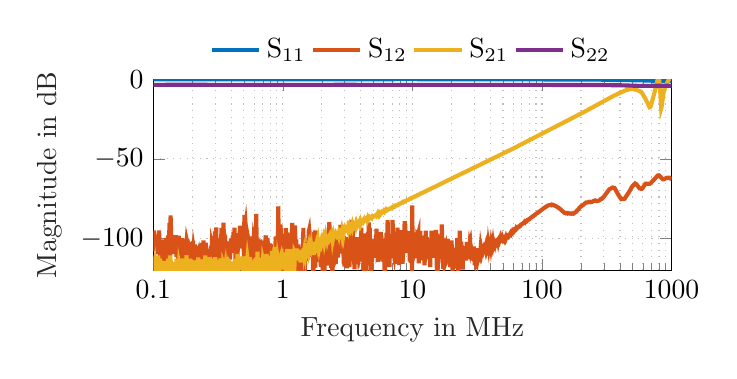
\begin{tikzpicture}

\begin{axis}[%
width=2.591in,
height=0.957in,
at={(0.616in,0.474in)},
scale only axis,
unbounded coords=jump,
xmode=log,
xmin=0.1,
xmax=1000,
xtick={0.1,1,10,100,1000},
xticklabels={{0.1},{1},{10},{100},{1000}},
xminorticks=true,
xlabel style={font=\color{white!15!black}},
xlabel={Frequency in MHz},
ymin=-120,
ymax=0,
ylabel style={font=\color{white!15!black}},
ylabel={Magnitude in dB},
axis background/.style={fill=white},
xmajorgrids,
xminorgrids,
ymajorgrids,
grid style={dotted},
legend style={at={(0.5,1.03)}, anchor=south, legend cell align=left, align=left, fill=none, draw=none},
legend columns = 4
]
\addplot [color=mycolor1, line width=1.5pt]
  table[row sep=crcr]{%
0.1	-0.08494777789\\
0.111287897	-0.06381854415\\
0.128925235	-0.0477322216\\
0.190228728	-0.01978593352\\
0.22243796	-0.01210351874\\
0.420798429	-0.01297250586\\
0.638028568	-0.03255212121\\
0.966623102	-0.03989368446\\
1.512860761	-0.0295475143\\
1.760803364	-0.02728326353\\
1.941905335	-0.02281109707\\
2.615863521	-0.01189003853\\
3.332085017	-0.006532293498\\
10.29337529	-0.003090868708\\
55.57604519	-0.03551824257\\
65.68848281	-0.05185938364\\
82.94119702	-0.07944399184\\
90.25694548	-0.1046574309\\
100.3684527	-0.1438726655\\
108.1007818	-0.193514553\\
121.6582671	-0.2797116816\\
127.3835643	-0.2907840068\\
138.8341588	-0.3039771395\\
149.4668536	-0.302402766\\
158.4637493	-0.2891425479\\
168.44499	-0.2558302997\\
183.1122813	-0.2164577989\\
195.5230661	-0.206008524\\
220.5378134	-0.2141800571\\
232.9848535	-0.2232333528\\
243.8760136	-0.2323570362\\
259.4348137	-0.2568018051\\
271.8818538	-0.2759805936\\
285.8847739	-0.3097288893\\
298.3318139	-0.3522713227\\
359.0634709	-0.579193023\\
369.7947792	-0.5760895638\\
378.3798258	-0.5680872791\\
389.111134	-0.5508425685\\
431.3651992	-0.5101273811\\
463.9222374	-0.5760820847\\
487.6000834	-0.6429482015\\
508.3181987	-0.6676058702\\
529.0363139	-0.6646727944\\
543.8349676	-0.6715468399\\
585.0287378	-0.7535595523\\
621.6579634	-0.8213916513\\
637.9376192	-0.8398170915\\
658.2871889	-0.8699993749\\
666.4270168	-0.8730854826\\
719.3358982	-0.9876411505\\
751.8952098	-0.9697579118\\
772.2447796	-0.9505024682\\
798.8918907	-0.9645904704\\
832.5773941	-1.025189036\\
849.4201459	-1.033472477\\
877.4913987	-1.057585165\\
899.948401	-1.110934959\\
933.6339044	-1.178946967\\
956.0909067	-1.170014164\\
1001.004911	-1.108793964\\
};
\addlegendentry{$\mathrm{S}_\mathrm{11}$}

\addplot [color=mycolor2, line width=1.5pt]
  table[row sep=crcr]{%
0.1	-101.6612071\\
0.100705494	-94.8785989\\
0.102821974	-101.27586\\
0.103527468	-107.9359009\\
0.104232961	-102.3117124\\
0.104938455	-104.2648978\\
0.105643948	-98.07594978\\
0.107054935	-101.8414036\\
0.107760429	-97.29833594\\
0.109171416	-109.865592\\
0.110582403	-94.92050723\\
0.11199339	-102.0464551\\
0.112698884	-118.5544446\\
0.114109871	-102.4881592\\
0.114815364	-106.4222965\\
0.116226351	-101.7188026\\
0.117637338	-114.6984546\\
0.119048325	-104.2106297\\
0.119753819	-107.7632023\\
0.121164806	-100.5862852\\
0.122575793	-114.1453393\\
0.125397767	-99.58742576\\
0.127514248	-114.3805469\\
0.128219741	-100.1750069\\
0.128925235	-114.1696017\\
0.129630728	-111.279501\\
0.130336222	-98.00774142\\
0.131041715	-107.8222415\\
0.131747209	-102.2000793\\
0.132452703	-104.3666805\\
0.133158196	-90.15176798\\
0.134569183	-114.5448114\\
0.13598017	-85.44126116\\
0.138482796	-106.9757777\\
0.13945599	-99.09841089\\
0.142375573	-109.6637692\\
0.144321962	-103.5260826\\
0.146268351	-107.5769702\\
0.147241545	-100.6422516\\
0.14821474	-103.6273466\\
0.149187934	-97.84236974\\
0.151134323	-111.3266106\\
0.152107517	-100.7546419\\
0.154053906	-107.8604267\\
0.156000295	-105.3050864\\
0.156973489	-98.12689212\\
0.159893073	-107.2059098\\
0.160866267	-103.2772305\\
0.161839461	-110.1420619\\
0.162812656	-108.1856152\\
0.16378585	-110.6905295\\
0.164759045	-102.6493369\\
0.166705433	-115.2561784\\
0.167678628	-99.66074861\\
0.169625017	-114.9751639\\
0.171571405	-103.1848466\\
0.1725446	-105.24554\\
0.173517794	-104.9671261\\
0.174490989	-108.3087905\\
0.175464183	-103.2153709\\
0.176437377	-112.5597271\\
0.177410572	-102.4059149\\
0.178383766	-105.0039582\\
0.179356961	-101.3338284\\
0.180330155	-103.5772632\\
0.181303349	-100.9374767\\
0.182276544	-101.7974904\\
0.183249738	-100.2750528\\
0.184222933	-103.9113956\\
0.185196127	-103.786561\\
0.187142516	-113.4240009\\
0.18811571	-102.186791\\
0.189088905	-121.4682761\\
0.190228728	-109.8559788\\
0.191570779	-120.7257083\\
0.195596933	-105.3913512\\
0.196938984	-113.7299849\\
0.198281036	-111.7092495\\
0.199623087	-112.9468109\\
0.200965139	-110.4555344\\
0.20230719	-101.4015351\\
0.203649241	-109.955907\\
0.204991293	-106.0392573\\
0.206333344	-107.5160974\\
0.207675395	-115.2583555\\
0.210359498	-103.5901069\\
0.21170155	-116.800467\\
0.213043601	-109.0132259\\
0.214385652	-116.5179234\\
0.215727704	-108.946324\\
0.217069755	-109.4147958\\
0.218411806	-106.5616134\\
0.219753858	-109.1012403\\
0.221095909	-108.4422565\\
0.223780012	-115.2372344\\
0.227806166	-107.4706251\\
0.229148217	-122.7604981\\
0.23183232	-104.6349932\\
0.235858474	-117.7653844\\
0.237200526	-102.709369\\
0.238542577	-112.526686\\
0.239884628	-104.763171\\
0.24122668	-109.5912505\\
0.243910782	-101.0933721\\
0.246594885	-113.7590798\\
0.247936937	-108.2890509\\
0.250621039	-114.4285217\\
0.251963091	-111.3181042\\
0.253305142	-121.9050319\\
0.254647193	-102.5679088\\
0.257331296	-111.9142703\\
0.258673347	-111.331246\\
0.260015399	-114.2040585\\
0.261582765	-107.360202\\
0.263428214	-107.5020559\\
0.265273664	-116.0202598\\
0.267119113	-106.4945288\\
0.268964563	-119.2758298\\
0.270810012	-109.3360673\\
0.272655462	-114.6228624\\
0.274500911	-111.841456\\
0.276346361	-116.1661646\\
0.28003726	-104.3817776\\
0.281882709	-120.435979\\
0.283728159	-103.2360943\\
0.289264507	-106.1131836\\
0.292955406	-99.71492346\\
0.294800856	-102.5397327\\
0.296646305	-111.2342414\\
0.298491755	-97.98847505\\
0.300337204	-98.19211174\\
0.302182654	-112.2336805\\
0.304028103	-108.5271888\\
0.305873553	-93.00490699\\
0.307719002	-104.8428976\\
0.309564452	-102.553979\\
0.311409901	-114.1308858\\
0.313255351	-113.5339321\\
0.3151008	-113.63197\\
0.31694625	-104.3036732\\
0.318791699	-116.6433139\\
0.320637149	-102.8836812\\
0.322482598	-109.3588883\\
0.324328048	-99.5292814\\
0.329864396	-126.1157632\\
0.331709845	-102.7666804\\
0.333555295	-111.2808764\\
0.335400744	-93.21671149\\
0.339091643	-104.6390812\\
0.340937093	-103.2868532\\
0.342782542	-111.1126326\\
0.344627992	-99.18359904\\
0.346473441	-102.1626595\\
0.348318891	-89.9521454\\
0.353855239	-114.1902839\\
0.355700689	-105.7639978\\
0.357546138	-106.5205824\\
0.359701417	-105.6619364\\
0.362247126	-117.7690484\\
0.364792835	-108.9807786\\
0.367338544	-109.2928804\\
0.369884252	-105.5101327\\
0.372429961	-107.4982904\\
0.37497567	-102.797493\\
0.377521379	-108.0571692\\
0.380067088	-103.3891853\\
0.385158505	-109.2451237\\
0.387704214	-101.7052375\\
0.390249923	-113.1233463\\
0.397887049	-99.92125498\\
0.402978467	-108.8985964\\
0.410615594	-98.23480597\\
0.413161302	-102.8414076\\
0.415707011	-95.8113723\\
0.41825272	-106.8934828\\
0.423344138	-93.0843018\\
0.425889847	-107.2157054\\
0.428435555	-97.59039635\\
0.430981264	-119.4429831\\
0.433526973	-102.5358366\\
0.436072682	-107.3504929\\
0.438618391	-96.75276099\\
0.441164099	-104.1422902\\
0.443709808	-100.1584479\\
0.446255517	-111.1372587\\
0.453892644	-96.64089548\\
0.456438352	-104.6221067\\
0.458984061	-101.9355951\\
0.464075479	-104.0367119\\
0.466621188	-91.8880371\\
0.469166896	-103.7367313\\
0.471712605	-91.95715903\\
0.476804023	-106.1179744\\
0.481895441	-99.22780957\\
0.486986858	-99.59287141\\
0.492078276	-93.52813371\\
0.497605565	-97.47608179\\
0.50111614	-114.9496427\\
0.504626715	-85.13613123\\
0.50813729	-94.24265263\\
0.515158441	-90.81627369\\
0.529200741	-105.0886603\\
0.532711316	-97.69507387\\
0.539732466	-109.3589565\\
0.543243041	-101.1216668\\
0.546753616	-102.3625923\\
0.557285342	-120.7496437\\
0.560795917	-109.3820687\\
0.564306492	-116.5504765\\
0.574838217	-98.64116888\\
0.578348792	-100.7868703\\
0.581859367	-114.0906098\\
0.595901667	-99.30397098\\
0.602922818	-101.3159065\\
0.606433393	-100.8512091\\
0.609943968	-109.27494\\
0.613454543	-102.5900117\\
0.620475693	-105.7532656\\
0.623986268	-84.40898006\\
0.627496843	-111.6659382\\
0.631007418	-108.4778324\\
0.634517993	-114.0148186\\
0.638028568	-113.6501026\\
0.641539144	-114.4578972\\
0.648560294	-104.8807268\\
0.652070869	-108.7657257\\
0.655581444	-107.524848\\
0.659092019	-108.8138671\\
0.662602594	-114.4019738\\
0.666113169	-111.9251818\\
0.669623744	-100.4310576\\
0.673134319	-111.8025576\\
0.680155469	-101.3168967\\
0.689098098	-114.4453232\\
0.693940768	-110.8939375\\
0.703626107	-117.6081808\\
0.708468776	-107.5225667\\
0.718154115	-112.8706322\\
0.737524793	-97.91549001\\
0.742367463	-113.1893364\\
0.747210132	-112.5329431\\
0.752052802	-99.58751765\\
0.756895471	-106.5684063\\
0.761738141	-99.51880832\\
0.77142348	-112.0097898\\
0.776266149	-124.4066757\\
0.785951488	-106.1627911\\
0.790794158	-118.7275916\\
0.795636827	-102.9728418\\
0.805322166	-118.1994042\\
0.829535514	-104.8780109\\
0.834378183	-104.9483937\\
0.839220853	-111.1078957\\
0.844063522	-104.3281472\\
0.848906192	-117.3312104\\
0.853748861	-106.4288601\\
0.858591531	-121.6850718\\
0.86827687	-104.138926\\
0.873119539	-106.0733291\\
0.882804878	-98.67503452\\
0.887647548	-102.3064327\\
0.892490217	-116.5908448\\
0.897332887	-116.5039929\\
0.911860895	-100.7014386\\
0.916703565	-101.7513915\\
0.921546234	-79.68948689\\
0.931231573	-108.6332877\\
0.936074243	-104.9776382\\
0.940916912	-105.5803392\\
0.946588735	-100.5502544\\
0.953266857	-105.7285206\\
0.95994498	-91.14533048\\
0.966623102	-99.62208779\\
0.973301224	-96.96128204\\
0.979979347	-100.9150776\\
0.986657469	-121.295123\\
1.000013714	-105.4552913\\
1.006691836	-116.7540222\\
1.026726203	-103.3731028\\
1.033404325	-99.31807701\\
1.040082447	-118.2036028\\
1.053438692	-93.36832519\\
1.060116814	-103.1343479\\
1.080151181	-96.15181055\\
1.093507426	-113.7842329\\
1.100185548	-99.65532977\\
1.10686367	-99.83022727\\
1.113541793	-96.84162401\\
1.126898037	-106.9903489\\
1.13357616	-104.9937687\\
1.140254282	-112.3659005\\
1.146932404	-98.12373782\\
1.160288649	-107.8301953\\
1.173644894	-100.0750701\\
1.180323016	-90.04635781\\
1.187001138	-106.029901\\
1.19367926	-105.3276541\\
1.200357383	-94.95149745\\
1.207035505	-106.8767356\\
1.213713627	-100.9326563\\
1.227069872	-115.9480065\\
1.240426117	-91.69193292\\
1.253782361	-106.7777703\\
1.267138606	-100.3946607\\
1.273816728	-126.667832\\
1.28049485	-105.3347343\\
1.301650396	-120.6046602\\
1.320016515	-103.5835034\\
1.347565693	-122.171248\\
1.365931811	-105.4120252\\
1.38429793	-115.6548101\\
1.393480989	-114.739042\\
1.402664049	-119.3514715\\
1.421030167	-112.3304659\\
1.430213227	-121.1018015\\
1.439396286	-93.23400334\\
1.448579346	-116.7473881\\
1.457762405	-108.0572577\\
1.476128524	-120.1496846\\
1.494494642	-104.8230805\\
1.512860761	-113.8649074\\
1.540409939	-102.175682\\
1.558776058	-112.9069552\\
1.586325236	-95.43602296\\
1.595508295	-94.56306651\\
1.604691355	-97.13674291\\
1.613874414	-110.737031\\
1.623057473	-100.7517152\\
1.632240533	-105.7825516\\
1.641423592	-99.62966539\\
1.650606652	-111.4860385\\
1.659789711	-103.491786\\
1.66897277	-107.9192679\\
1.67815583	-96.83250118\\
1.687338889	-98.64600836\\
1.696521948	-98.31849037\\
1.705705008	-101.2407837\\
1.714092258	-132\\
nan	nan\\
1.715957292	-132\\
1.733254186	-107.5117483\\
1.742437245	-118.2701068\\
1.751620305	-98.54304847\\
1.779169483	-118.1402345\\
1.78989427	-94.89760583\\
1.815229447	-114.62402\\
1.827897036	-104.5264876\\
1.840564625	-113.1851322\\
1.865899803	-102.3487165\\
1.878567391	-107.6913838\\
1.89123498	-105.2558158\\
1.903902569	-108.8253338\\
1.929237746	-105.0526727\\
1.967240513	-117.6789349\\
1.979908101	-113.2694856\\
1.99257569	-113.4092697\\
2.017910868	-107.8418873\\
2.030578457	-125.4356815\\
2.043246045	-104.6705185\\
2.055913634	-113.4173612\\
2.081248812	-107.5012669\\
2.0939164	-121.1066623\\
2.106583989	-110.5502876\\
2.119251578	-113.6600291\\
2.131919167	-108.5428533\\
2.144586756	-109.7493881\\
2.157254344	-115.0160707\\
2.169921933	-97.20575189\\
2.182589522	-116.8545986\\
2.195257111	-97.47708149\\
2.220592288	-108.2491519\\
2.245927466	-97.79258247\\
2.258595054	-98.14812894\\
2.271262643	-100.2732178\\
2.283930232	-89.68309428\\
2.321932998	-106.5879371\\
2.334600587	-98.09161174\\
2.359935765	-118.2835156\\
2.372603353	-99.21269034\\
2.385270942	-110.1855144\\
2.397938531	-104.0295084\\
2.41060612	-129.3484787\\
2.423273708	-108.60506\\
2.435941297	-116.3109231\\
2.448608886	-108.6022804\\
2.461276475	-115.8396962\\
2.476112985	-107.214084\\
2.493581802	-115.3792825\\
2.511050619	-99.04574498\\
2.528519436	-103.6366552\\
2.545988253	-102.0061915\\
2.56345707	-115.8881333\\
2.580925887	-103.0835392\\
2.598394704	-110.0479646\\
2.615863521	-109.2701305\\
2.633332338	-103.2463964\\
2.650801155	-111.7915801\\
2.668269972	-97.76505235\\
2.703207606	-103.7130365\\
2.720676423	-109.3809038\\
2.773082874	-91.35160165\\
2.825489325	-99.06668974\\
2.842958142	-97.70239067\\
2.860426959	-99.59607878\\
2.877895776	-91.80677018\\
2.91283341	-103.3407709\\
2.930302227	-101.4071959\\
2.947771044	-115.6779714\\
2.965239861	-98.26675289\\
2.982708678	-117.5273151\\
3.017646312	-99.75314278\\
3.070052763	-107.5451135\\
3.087521579	-104.645573\\
3.122459213	-118.5783893\\
3.157396847	-106.6326148\\
3.174865664	-109.5063073\\
3.192334481	-99.04909589\\
3.227272115	-107.3166827\\
3.244740932	-106.6298424\\
3.262209749	-117.8064074\\
3.3146162	-95.94384318\\
3.332085017	-102.4172653\\
3.349553834	-93.30650327\\
3.367022651	-100.384347\\
3.384491468	-88.20912661\\
3.428914395	-114.265592\\
3.452935696	-92.11570351\\
3.476956996	-105.7217428\\
3.500978297	-98.97428362\\
3.573042199	-119.2342003\\
3.597063499	-106.6871057\\
3.6210848	-111.0088461\\
3.6451061	-103.6163222\\
3.693148702	-110.1934606\\
3.717170002	-102.9762172\\
3.765212603	-115.94097\\
3.789233904	-99.06026635\\
3.837276505	-107.4676069\\
3.861297806	-103.0734989\\
3.885319106	-110.3613093\\
3.909340407	-109.3039568\\
3.933361707	-105.0224303\\
3.957383008	-108.811075\\
3.981404309	-107.7622765\\
4.02944691	-93.12343303\\
4.077489511	-114.2024388\\
4.101510811	-107.9312457\\
4.125532112	-109.5871665\\
4.149553413	-101.7440129\\
4.197596014	-115.4184579\\
4.245638615	-113.7482639\\
4.293681216	-96.71224207\\
4.413787719	-121.8183441\\
4.46183032	-103.1617245\\
4.485851621	-112.1176604\\
4.533894222	-95.76278425\\
4.581936823	-108.1508732\\
4.605958124	-89.82498888\\
4.629979424	-97.48164205\\
4.654000725	-93.71886426\\
4.68205492	-93.89988666\\
4.715191149	-108.4771105\\
4.748327378	-106.4120748\\
4.814599836	-120.8843338\\
4.847736065	-107.4582186\\
4.880872294	-114.5598757\\
4.914008523	-106.7612804\\
4.947144752	-107.1024501\\
5.01341721	-111.2826342\\
5.046553439	-103.3517742\\
5.112825896	-103.8553252\\
5.145962125	-100.3996974\\
5.179098354	-103.2788227\\
5.212234583	-112.0334158\\
5.278507041	-93.78746265\\
5.31164327	-105.3256563\\
5.344779499	-99.91741923\\
5.377915728	-110.0986425\\
5.411051957	-109.6307015\\
5.444188186	-114.45578\\
5.477324415	-99.91795672\\
5.543596873	-110.7582292\\
5.576733102	-108.2245195\\
5.609869331	-100.133739\\
5.64300556	-108.5800691\\
5.709278018	-95.81179531\\
5.742414247	-107.2316231\\
5.775550475	-105.8530457\\
5.808686704	-113.6709689\\
5.841822933	-100.5334289\\
5.908095391	-113.1586441\\
5.94123162	-106.7090858\\
5.974367849	-114.5873621\\
6.040640307	-105.8378237\\
6.073776536	-106.5615391\\
6.106912765	-129.0377313\\
6.206321452	-102.5786672\\
6.239457681	-109.6340521\\
6.305730139	-96.38616112\\
6.338866368	-110.4899403\\
6.438275055	-88.35077054\\
6.522780223	-113.5669808\\
6.568475638	-105.5568646\\
6.659866467	-117.8102937\\
6.705561881	-102.3679221\\
6.751257296	-106.1272592\\
6.79695271	-98.88715862\\
6.842648125	-104.2679969\\
6.934038953	-99.1833943\\
6.979734368	-102.5773701\\
7.025429782	-88.23815368\\
7.162516026	-109.5783177\\
7.20821144	-110.8542378\\
7.345297683	-102.3795338\\
7.390993098	-115.7589616\\
7.436688512	-101.9978249\\
7.482383927	-108.3876512\\
7.573774756	-96.22600056\\
7.61947017	-100.367001\\
7.665165585	-93.1781027\\
7.756556413	-113.6876601\\
7.802251828	-108.306182\\
7.847947242	-108.4922838\\
7.893642657	-116.5043678\\
8.076424314	-94.67013891\\
8.122119729	-109.0171549\\
8.167815143	-100.1546015\\
8.213510558	-110.067169\\
8.259205972	-100.4014449\\
8.396292216	-115.686366\\
8.533378459	-101.9990552\\
8.579073873	-104.0984995\\
8.716160117	-89.04459924\\
8.761855531	-99.26101731\\
8.807550946	-90.91074209\\
8.906613499	-106.0630155\\
8.969648125	-103.9935155\\
9.095717379	-108.8899114\\
9.158752005	-100.1031669\\
9.221786632	-104.4196663\\
9.284821259	-95.27882412\\
9.347855886	-108.717368\\
9.473925139	-103.7282827\\
9.536959766	-114.1774038\\
9.599994392	-110.6800413\\
9.726063646	-115.0625594\\
9.852132899	-96.91591896\\
9.915167526	-120.6154626\\
9.978202153	-79.17761818\\
10.04123678	-114.1957836\\
10.10427141	-98.65492441\\
10.16730603	-110.3464496\\
10.29337529	-96.17887111\\
10.35640991	-97.98211288\\
10.41944454	-107.6858531\\
10.48247917	-98.24816695\\
10.67158305	-112.3314581\\
10.73461767	-100.419353\\
10.7976523	-108.361505\\
10.86068693	-106.4717595\\
10.92372155	-97.83952019\\
10.98675618	-98.14005421\\
11.11282543	-96.59094395\\
11.17586006	-115.4590295\\
11.30192931	-102.0600753\\
11.42799857	-105.2350236\\
11.49103319	-95.21098875\\
11.61710245	-110.5674412\\
11.68013707	-99.19276181\\
11.7431717	-99.58701922\\
11.93227558	-113.5383673\\
12.05834483	-104.3559816\\
12.18441409	-112.66379\\
12.32127602	-98.20741977\\
12.40820182	-116.7156047\\
12.66897924	-94.99450558\\
12.75590504	-112.8638988\\
12.92975665	-99.13811675\\
13.10360827	-110.8722223\\
13.19053407	-103.9992695\\
13.27745988	-109.4586384\\
13.53823729	-102.0637911\\
13.6251631	-104.7284586\\
13.7120889	-117.8119106\\
13.79901471	-107.0103981\\
13.88594051	-108.825329\\
14.05979212	-94.94071039\\
14.14671793	-107.2540056\\
14.23364374	-107.1734913\\
14.32056954	-112.0519359\\
14.58134696	-98.83079653\\
14.66827276	-106.5847982\\
14.75519857	-103.8274656\\
14.84212437	-109.6945021\\
14.92905018	-104.6092552\\
15.01597599	-109.8593467\\
15.1898276	-94.53993593\\
15.2767534	-107.147398\\
15.36367921	-96.49002824\\
15.45060501	-123.7903751\\
15.53753082	-102.4326277\\
15.79830823	-107.0945268\\
15.97215985	-110.126685\\
16.14601146	-105.1778257\\
16.23293726	-112.6470748\\
16.31986307	-97.31095132\\
16.58064048	-110.0980286\\
16.66756629	-107.6756967\\
16.75449209	-108.016128\\
16.8414179	-91.03646044\\
17.30153151	-118.8246582\\
17.54059417	-99.90553925\\
17.77965683	-116.440948\\
17.89918816	-115.7154821\\
18.01871949	-101.0428446\\
18.13825081	-105.5797933\\
18.25778214	-104.4250441\\
18.4968448	-106.8727658\\
18.73590746	-100.2072051\\
18.85543878	-108.2494836\\
18.97497011	-103.6292449\\
19.21403277	-107.1178106\\
19.3335641	-104.9517919\\
19.45309543	-105.4194815\\
19.57262676	-117.7539499\\
19.81168941	-104.7538898\\
19.93122074	-113.7521473\\
20.05075207	-101.15127\\
20.40934606	-122.0105319\\
20.64840871	-107.5941375\\
20.76794004	-114.9070785\\
20.88747137	-108.8609063\\
21.0070027	-118.7620725\\
21.12653403	-112.0682226\\
21.24606536	-115.942327\\
21.48512801	-105.6372792\\
21.843722	-113.7093229\\
22.20231598	-99.4927125\\
22.32184731	-112.494519\\
22.44137864	-104.2169244\\
22.56090997	-126.2674002\\
22.6804413	-103.8460158\\
22.79997263	-108.2534416\\
22.91950396	-107.9752571\\
23.03903528	-110.9170934\\
23.15856661	-94.97768888\\
23.46305357	-109.3930306\\
23.62794129	-108.9151235\\
23.79282901	-101.9811185\\
24.45237988	-119.310564\\
24.6172676	-106.2480816\\
24.78215532	-106.6630711\\
25.11193076	-113.3735322\\
25.27681848	-104.6941755\\
25.4417062	-110.9461558\\
25.60659392	-107.5366921\\
25.77148164	-113.6769532\\
26.10125708	-107.5191742\\
26.2661448	-102.1182393\\
26.43103252	-103.6990618\\
26.59592024	-112.8403147\\
26.92569567	-105.0440112\\
27.25547111	-111.4271607\\
27.58524655	-105.4606154\\
27.91502199	-107.8375376\\
28.07990971	-106.5184047\\
28.24479743	-110.3487762\\
28.40968515	-106.0394507\\
28.73946059	-108.3490829\\
28.90434831	-108.104468\\
29.06923603	-109.0409062\\
29.23412375	-113.202978\\
29.39901147	-107.015248\\
29.56389918	-113.9411139\\
29.7287869	-104.846978\\
29.89367462	-108.3745322\\
30.05856234	-106.9395501\\
30.22345006	-116.7853864\\
30.38833778	-108.6304214\\
30.5532255	-111.791273\\
30.71811322	-109.0691249\\
30.88300094	-112.0091891\\
31.04788866	-110.8010182\\
31.21277638	-106.0619384\\
31.70743954	-110.803359\\
32.03721498	-107.0385847\\
32.23033447	-109.8877472\\
32.4577174	-109.6107743\\
32.68510032	-109.9459456\\
32.91248325	-106.1187877\\
33.13986618	-110.2299602\\
33.3672491	-109.4816504\\
33.59463202	-106.5400968\\
33.82201495	-108.306775\\
34.04939788	-107.1179618\\
34.2767808	-108.5659613\\
34.73154665	-106.1580223\\
34.95892958	-106.5306693\\
35.1863125	-106.0100327\\
35.41369543	-107.0590683\\
35.64107835	-106.2958804\\
36.0958442	-106.6889623\\
36.32322713	-106.1788923\\
36.77799298	-104.5349986\\
37.00537591	-106.0329288\\
37.23275883	-105.0204635\\
37.46014176	-106.8855191\\
38.14229053	-104.6691094\\
38.36967346	-106.9219168\\
38.59705638	-104.1661927\\
38.82443931	-105.6679337\\
39.05182223	-104.0994568\\
39.50658808	-105.0367872\\
39.73397101	-104.6152622\\
39.96135393	-104.7662279\\
40.18873686	-103.4314099\\
40.41611978	-104.9717438\\
40.64350271	-103.5292152\\
41.09826856	-103.9593829\\
41.32565149	-104.6689013\\
41.78041734	-102.2761501\\
42.00780026	-103.6961618\\
42.46256611	-101.8472329\\
43.14471489	-103.6294157\\
43.37209781	-102.5152591\\
44.05424659	-103.3120725\\
44.94515115	-101.3511741\\
45.2578245	-101.5116992\\
45.57049786	-101.1035653\\
45.88317121	-102.2664995\\
46.19584457	-101.0774556\\
46.50851792	-101.2147604\\
46.82119127	-101.6526277\\
47.44653798	-100.0931103\\
47.75921134	-101.3266456\\
48.07188469	-101.2348898\\
48.38455805	-100.4460458\\
48.6972314	-100.7024511\\
49.00990475	-100.1610526\\
49.32257811	-100.3100495\\
49.63525146	-99.2909337\\
50.26059817	-100.4108449\\
50.88594488	-99.6328454\\
51.19861823	-99.67734571\\
51.51129158	-99.38548699\\
51.82396494	-100.160465\\
52.44931165	-99.06935956\\
52.761985	-99.84824326\\
53.07465836	-99.28858595\\
53.38733171	-99.33707219\\
53.70000506	-99.31025665\\
54.95069848	-97.89353759\\
55.26337183	-97.92800339\\
55.57604519	-98.29212309\\
56.82673861	-96.86939135\\
57.45208531	-97.2277222\\
58.07743202	-96.06807893\\
58.39010537	-96.23770033\\
58.70277873	-95.85235838\\
59.01545208	-96.04468155\\
59.32812544	-95.5773921\\
59.64079879	-95.89524692\\
60.57881885	-94.96922826\\
60.9439864	-95.2910147\\
62.23793996	-94.20686578\\
62.66925782	-94.22613506\\
63.10057567	-93.57641816\\
63.53189353	-93.9252637\\
65.25716495	-92.74989544\\
65.68848281	-92.81842678\\
67.41375423	-91.90707538\\
67.84507208	-92.04495189\\
69.5703435	-91.00211221\\
70.00166136	-90.95861018\\
72.58956849	-89.7931196\\
73.02088635	-89.8051049\\
73.4522042	-89.91403178\\
73.88352206	-89.43367331\\
74.31483991	-89.59847791\\
76.04011133	-88.77874862\\
76.47142919	-88.9385499\\
78.19670061	-88.08802537\\
78.62801846	-88.10550136\\
79.92197203	-87.61382803\\
80.35328989	-87.62296724\\
81.2159256	-87.18866782\\
84.90379459	-85.96083311\\
85.49858914	-85.99086627\\
89.0673564	-84.69301645\\
93.82571274	-83.47773495\\
104.5320145	-80.56635809\\
105.1268091	-80.51919943\\
109.2903709	-79.5626656\\
110.4799599	-79.36229491\\
113.4539327	-78.98699666\\
117.5687691	-78.73627334\\
118.3866687	-78.8812736\\
119.2045683	-78.64750775\\
120.8403675	-78.80939161\\
121.6582671	-78.79335567\\
128.2014639	-79.60931049\\
133.9267612	-80.59658017\\
136.38046	-81.01996271\\
144.559456	-82.83481807\\
149.4668536	-83.82995802\\
150.2847533	-83.82033781\\
152.7384521	-84.08556674\\
153.5563517	-83.98193853\\
156.0100505	-84.05377162\\
156.8279501	-83.87643715\\
157.6458497	-83.90614163\\
158.4637493	-84.08618021\\
159.4189647	-83.92054434\\
165.0602305	-84.31234484\\
166.1884837	-84.22001499\\
167.3167369	-84.24206679\\
168.44499	-84.22905207\\
169.5732432	-84.3587924\\
170.7014964	-84.3256599\\
171.8297495	-84.14946652\\
172.9580027	-84.19132324\\
174.0862559	-84.14447632\\
175.2145091	-84.26942463\\
183.1122813	-83.20604275\\
186.4970408	-82.35059072\\
187.6252939	-82.37407314\\
195.5230661	-80.44372545\\
205.6773447	-79.04913421\\
206.8055979	-79.01875265\\
218.0881296	-77.39761861\\
219.2163827	-77.43718221\\
225.2054534	-77.23102298\\
228.3172134	-77.06551828\\
231.4289735	-76.86595708\\
234.5407335	-76.97772465\\
236.0966135	-77.11189616\\
239.2083735	-77.06699637\\
242.3201335	-76.98471233\\
251.6554136	-76.21513566\\
256.3230536	-76.02832066\\
257.8789337	-76.17835622\\
259.4348137	-76.17211061\\
262.5465737	-76.36780139\\
264.1024537	-76.35977642\\
267.2142137	-76.40681633\\
276.5494938	-76.04115399\\
284.3288938	-75.19069979\\
285.8847739	-75.28520874\\
290.5524139	-75.00582921\\
299.8876939	-73.68312982\\
331.1620695	-69.06340737\\
333.3083311	-69.00940063\\
350.4784243	-67.90756263\\
352.624686	-67.92493788\\
363.3559942	-68.23847276\\
391.2573957	-72.8910427\\
408.4274889	-75.13569435\\
414.8662739	-74.98693341\\
419.5262762	-75.00290453\\
425.4457377	-75.08752041\\
431.3651992	-75.06059951\\
434.32493	-74.97628633\\
472.8014297	-70.38934215\\
496.4792757	-67.32807623\\
523.1168524	-65.37637225\\
534.9557754	-65.80373176\\
543.8349676	-66.55667533\\
564.5530828	-68.31971847\\
567.5128136	-68.2857415\\
580.9588239	-68.78292457\\
589.0986518	-68.7257736\\
597.2384797	-68.32351788\\
629.7977913	-65.48579592\\
633.8677052	-65.46799769\\
646.0774471	-65.6412822\\
650.147361	-65.548995\\
658.2871889	-65.63128947\\
662.3571029	-65.60301505\\
670.4969308	-65.67931347\\
678.6367587	-65.66275362\\
690.8465005	-65.19376784\\
784.4545214	-60.34054093\\
788.5244354	-60.35433918\\
798.8918907	-60.28447549\\
810.1203919	-60.65710398\\
838.1916447	-62.06218742\\
855.0343964	-62.71919512\\
860.648647	-62.66024028\\
866.2628976	-62.77536966\\
877.4913987	-62.68875334\\
899.948401	-62.1633358\\
928.0196538	-61.79197086\\
939.248155	-61.91216733\\
944.8624056	-61.89867281\\
950.4766561	-61.82755147\\
967.3194078	-61.84335266\\
972.9336584	-61.9122999\\
1001.004911	-62.88776028\\
};
\addlegendentry{$\mathrm{S}_\mathrm{12}$}

\addplot [color=mycolor3, line width=1.5pt]
  table[row sep=crcr]{%
0.1	-118.789\\
0.101410987	-116.2463076\\
0.102116481	-123.2575473\\
0.102821974	-113.6630672\\
0.104232961	-124.5129106\\
0.104938455	-115.6496852\\
0.105643948	-118.4375033\\
0.107054935	-111.0413339\\
0.107760429	-119.2727754\\
0.109171416	-110.546873\\
0.109876909	-118.5864691\\
0.110582403	-113.631229\\
0.111287897	-122.7816925\\
0.11199339	-112.3935505\\
0.112698884	-123.324442\\
0.114815364	-113.7626544\\
0.116931845	-124.0081432\\
0.117637338	-114.3541582\\
0.119048325	-124.8472824\\
0.120459312	-115.1719509\\
0.121164806	-119.8101436\\
0.1218703	-118.5137648\\
0.122575793	-114.1479276\\
0.12398678	-120.2509548\\
0.124692274	-116.114321\\
0.126103261	-120.6032986\\
0.126808754	-117.4598589\\
0.127514248	-119.8312732\\
0.128219741	-115.6514933\\
0.128925235	-119.9159082\\
0.129630728	-112.6148923\\
0.131041715	-123.002659\\
0.131747209	-114.027787\\
0.133158196	-119.5826902\\
0.134569183	-110.4879076\\
0.13598017	-118.2544225\\
0.136685664	-113.7588499\\
0.137509601	-116.8414394\\
0.138482796	-129.161663\\
0.13945599	-118.5341909\\
0.140429185	-125.7051239\\
0.141402379	-114.6302122\\
0.142375573	-123.8050634\\
0.143348768	-119.3036111\\
0.144321962	-126.5544627\\
0.145295157	-116.9653739\\
0.146268351	-121.8868975\\
nan	nan\\
0.14821474	-125.2794524\\
0.151134323	-112.5851495\\
0.152107517	-126.3670871\\
0.153080712	-119.6480585\\
0.154053906	-125.471174\\
0.155027101	-119.2878361\\
0.156000295	-124.1731342\\
0.157946684	-116.2800624\\
0.158919878	-117.5170284\\
0.159893073	-112.5446546\\
0.160866267	-121.9275464\\
0.161839461	-118.8285206\\
0.162812656	-122.6643626\\
0.16378585	-117.8538123\\
0.164759045	-127.5828622\\
0.166705433	-115.8288632\\
0.1673876028	-132\\
nan	nan\\
0.1679309286	-132\\
0.168651822	-112.4020423\\
0.170598211	-118.3824537\\
0.171571405	-114.3363326\\
0.1725446	-125.2810175\\
0.173517794	-117.4388546\\
0.174490989	-125.3924307\\
0.175464183	-116.4102673\\
0.176437377	-119.4544365\\
0.177410572	-115.1412844\\
0.178383766	-117.9695577\\
0.1789924584	-132\\
nan	nan\\
0.1796279289	-132\\
0.180330155	-110.3440767\\
0.181303349	-125.8988977\\
0.182276544	-119.3508045\\
0.183249738	-128.945547\\
0.184222933	-117.7377629\\
0.185196127	-119.1638555\\
0.186169321	-131.0845078\\
0.187142516	-113.5111379\\
0.190228728	-120.1400136\\
0.191570779	-112.5682317\\
0.1940452057	-132\\
nan	nan\\
0.1944058412	-132\\
0.195596933	-113.053812\\
0.196938984	-122.8779267\\
0.199623087	-117.0013058\\
0.200965139	-119.9789836\\
0.20230719	-113.6895916\\
0.205988812	-132\\
nan	nan\\
0.2065831672	-132\\
0.207675395	-118.4605286\\
0.209017447	-126.8671871\\
0.21170155	-117.0286721\\
0.213043601	-121.7378407\\
0.214385652	-121.3769328\\
0.215727704	-119.7405767\\
0.217069755	-113.5150885\\
0.219753858	-123.3299151\\
0.22243796	-111.7414957\\
0.223780012	-124.8774032\\
0.226464115	-116.105298\\
0.227806166	-125.0133419\\
0.229148217	-119.6354478\\
0.230490269	-120.1746962\\
nan	nan\\
0.233174371	-121.1734112\\
0.234516423	-119.4500824\\
0.2355703131	-132\\
nan	nan\\
0.2361070922	-132\\
0.238542577	-112.9968837\\
0.24122668	-116.0295837\\
0.242568731	-124.8768222\\
nan	nan\\
0.2456902822	-132\\
0.246594885	-113.8161377\\
0.250621039	-119.8540143\\
0.251963091	-110.5380571\\
0.253305142	-124.8544832\\
0.254647193	-117.643514\\
0.255989245	-119.8217108\\
0.257331296	-119.6198224\\
0.258673347	-128.381002\\
0.260015399	-118.5560861\\
0.263428214	-123.2576652\\
0.265273664	-114.1886069\\
0.267119113	-120.3779045\\
0.268964563	-116.0190949\\
0.270810012	-119.4039782\\
0.272655462	-111.6032154\\
0.274500911	-118.9467191\\
0.276346361	-113.1248401\\
0.2781477964	-132\\
nan	nan\\
0.2782509695	-132\\
0.281882709	-117.0944922\\
0.283728159	-120.106694\\
0.285573608	-129.556935\\
0.287419058	-119.0434938\\
0.291109957	-120.5992076\\
0.2928649407	-132\\
nan	nan\\
0.2930344716	-132\\
0.296646305	-112.3884845\\
0.298491755	-119.4842923\\
0.300337204	-111.6178239\\
0.302182654	-119.6240243\\
0.304028103	-114.8084637\\
0.307719002	-125.8156067\\
0.311409901	-113.1602992\\
0.313255351	-115.6273404\\
0.3151008	-113.6634546\\
0.31694625	-118.401032\\
0.318791699	-113.403441\\
0.320637149	-126.7227773\\
nan	nan\\
0.324328048	-120.5800534\\
0.331709845	-112.3718867\\
0.333555295	-118.0898142\\
0.337246194	-115.5109472\\
0.339091643	-125.108002\\
0.340937093	-114.9091092\\
0.342782542	-126.8389912\\
0.346473441	-115.1827695\\
0.35016434	-116.2695498\\
0.35200979	-119.6774834\\
0.353855239	-118.6469841\\
0.355700689	-112.3944307\\
0.357546138	-117.7619163\\
0.359701417	-116.4225639\\
0.362247126	-119.3194753\\
0.364792835	-117.344816\\
0.367338544	-123.0506455\\
0.369884252	-122.2486552\\
0.372429961	-115.3753541\\
0.37497567	-122.4776785\\
0.380067088	-118.6445029\\
0.382612797	-122.0087553\\
0.385158505	-114.4615432\\
0.387704214	-114.8122526\\
0.390249923	-116.9587186\\
0.392795632	-116.7740122\\
0.395341341	-119.7313648\\
0.400432758	-114.4847311\\
0.405524176	-124.6933719\\
0.408069885	-119.9674798\\
0.410615594	-130.5803191\\
nan	nan\\
0.41825272	-124.1083792\\
0.420798429	-117.8894534\\
0.423344138	-119.538631\\
0.425889847	-113.8147905\\
0.428435555	-115.2142254\\
0.430981264	-112.6112263\\
0.433526973	-121.7021073\\
0.438618391	-115.7554755\\
0.441164099	-128.1156573\\
0.443709808	-125.3303376\\
0.446255517	-109.5750494\\
0.448801226	-113.271251\\
0.451346935	-125.7786989\\
0.453892644	-115.5513212\\
0.456438352	-118.2135371\\
0.458984061	-116.869133\\
0.46152977	-111.837481\\
0.464075479	-119.2755389\\
0.466621188	-112.6226319\\
0.471712605	-119.0594832\\
0.474258314	-113.3733456\\
0.481895441	-119.116268\\
0.484441149	-111.1641984\\
0.486986858	-118.6049751\\
0.489532567	-113.5110103\\
0.492078276	-120.1067017\\
0.494623985	-118.3465037\\
0.497605565	-123.0247505\\
0.504626715	-114.7884405\\
0.50813729	-120.3510668\\
nan	nan\\
0.515158441	-121.4584761\\
0.522179591	-110.9884572\\
0.525690166	-116.6868955\\
0.532711316	-111.6822597\\
0.539732466	-115.125972\\
0.543243041	-130.5903006\\
0.550264191	-113.7234109\\
0.553774767	-129.6489742\\
0.557285342	-111.6745509\\
0.571327642	-129.2910758\\
0.574838217	-118.0401637\\
0.578348792	-120.6439017\\
0.581859367	-114.4923226\\
0.588880517	-123.5431174\\
0.592391092	-116.2765507\\
0.595901667	-123.8656762\\
0.606433393	-112.9911212\\
0.609943968	-126.3659563\\
0.616965118	-112.2694044\\
0.620475693	-120.386896\\
0.627496843	-111.6077706\\
0.634517993	-121.9715201\\
0.638028568	-108.127921\\
0.641539144	-125.7791664\\
0.645049719	-117.2981116\\
0.648560294	-125.0558906\\
0.655581444	-112.9822796\\
0.6587273752	-132\\
nan	nan\\
0.6594709759	-132\\
0.666113169	-111.9702509\\
0.669623744	-117.7518119\\
0.673134319	-112.7157462\\
0.680155469	-129.9456804\\
nan	nan\\
0.6892581873	-132\\
0.703626107	-113.2389947\\
0.708468776	-114.2538515\\
0.712732812	-132\\
nan	nan\\
0.7138023311	-132\\
0.718154115	-110.7955899\\
0.722996785	-122.8863866\\
0.732682124	-115.0528434\\
0.742367463	-122.3113835\\
0.747210132	-109.6429714\\
0.752052802	-111.1412072\\
0.7574936241	-132\\
0.761738141	-110.6468744\\
0.76658081	-122.650623\\
0.77142348	-111.5647677\\
0.776266149	-113.4105924\\
0.781108819	-123.2854894\\
0.790794158	-113.1093238\\
0.805322166	-120.4839325\\
0.810164836	-112.1320359\\
0.819850175	-126.9039505\\
0.824692844	-107.5951647\\
0.829535514	-115.7451523\\
0.834378183	-114.5039875\\
0.839220853	-119.9013959\\
0.844063522	-113.1222234\\
0.848906192	-117.6057074\\
0.8634342	-105.2927814\\
0.873119539	-120.1891885\\
0.877962209	-114.8063906\\
0.882804878	-115.7430996\\
0.887647548	-114.9026293\\
0.892490217	-110.653021\\
0.897332887	-126.7158267\\
0.907018226	-109.8469887\\
0.911860895	-116.7886473\\
0.916703565	-112.6533445\\
0.921546234	-113.7489989\\
0.926388904	-119.9941096\\
0.931231573	-112.3675484\\
0.936163408	-132\\
0.940916912	-113.5517453\\
0.946588735	-113.6322325\\
0.95994498	-111.8420598\\
0.973301224	-119.3323178\\
0.979979347	-114.9927081\\
0.993335591	-112.7719828\\
1.006691836	-116.2456995\\
1.013369958	-116.047058\\
1.033404325	-108.6706082\\
1.053438692	-120.0827988\\
1.060116814	-112.5174808\\
1.066794937	-117.5029215\\
1.080151181	-106.473361\\
1.113541793	-117.9787976\\
1.120219915	-110.5877932\\
1.13357616	-121.3482353\\
1.153610527	-106.5444258\\
1.166966771	-113.0766442\\
1.173644894	-109.6916037\\
1.180323016	-109.7777976\\
1.187001138	-113.4364588\\
1.19367926	-108.5195002\\
1.200357383	-111.7561943\\
1.207035505	-111.403899\\
1.213713627	-112.5261605\\
1.22039175	-129.79874\\
1.233747994	-108.4791462\\
1.247104239	-109.2895113\\
1.253782361	-113.4303217\\
1.273816728	-106.1370772\\
1.28049485	-111.5404659\\
1.287172973	-106.5214446\\
1.301650396	-108.9745805\\
1.310833455	-108.8869388\\
1.320016515	-113.6771303\\
1.329199574	-107.9525186\\
1.338382633	-110.5498521\\
1.347565693	-110.4221215\\
1.356748752	-107.4988825\\
1.365931811	-114.9385218\\
1.375114871	-108.0065704\\
1.38429793	-111.5102884\\
1.402664049	-107.0271506\\
1.411847108	-110.9263049\\
1.421030167	-107.558799\\
1.430213227	-110.7398014\\
1.448579346	-106.0253373\\
1.457762405	-108.7455268\\
1.466945464	-107.2203812\\
1.476128524	-108.5095755\\
1.485311583	-105.6111757\\
1.494494642	-107.6718209\\
1.503677702	-105.4901384\\
1.52204382	-110.1604078\\
1.53122688	-106.1517972\\
1.540409939	-109.3334095\\
1.549592999	-102.867104\\
1.558776058	-105.9398209\\
1.577142177	-104.2969769\\
1.595508295	-108.0788354\\
1.623057473	-105.3131236\\
1.641423592	-106.3943755\\
1.650606652	-105.0538452\\
1.659789711	-107.3222668\\
1.66897277	-104.49662\\
1.67815583	-107.591597\\
1.687338889	-104.6319545\\
1.696521948	-105.1237977\\
1.705705008	-101.8755085\\
1.714888067	-106.5558578\\
1.724071126	-102.546595\\
1.733254186	-110.0594317\\
1.751620305	-102.5533958\\
1.769986423	-108.9165649\\
1.802561859	-103.2710778\\
1.815229447	-103.1299632\\
1.827897036	-102.0266323\\
1.853232214	-103.4208774\\
1.865899803	-101.9594956\\
1.878567391	-104.07667\\
1.903902569	-101.9870364\\
1.916570158	-99.30361441\\
1.929237746	-103.8443217\\
1.941905335	-102.638144\\
1.954572924	-102.744127\\
1.967240513	-103.1644856\\
1.979908101	-102.0064452\\
1.99257569	-103.0846137\\
2.030578457	-100.6602816\\
2.043246045	-103.5454027\\
2.055913634	-100.9191328\\
2.068581223	-101.3068495\\
2.081248812	-100.5204268\\
2.0939164	-102.1724013\\
2.119251578	-99.88931355\\
2.131919167	-101.8879339\\
2.144586756	-101.5892818\\
2.169921933	-98.67360991\\
2.182589522	-98.98929811\\
2.195257111	-101.6679321\\
2.207924699	-98.45985296\\
2.220592288	-100.5241582\\
2.233259877	-99.75245108\\
2.245927466	-99.85504743\\
2.296597821	-98.12949344\\
2.30926541	-99.13523223\\
2.321932998	-98.60970595\\
2.359935765	-99.90077237\\
2.372603353	-99.27434576\\
2.385270942	-99.49871213\\
2.397938531	-99.33519272\\
2.41060612	-97.54179118\\
2.423273708	-99.69612775\\
2.435941297	-98.47789588\\
2.448608886	-99.02313353\\
2.461276475	-97.97429457\\
2.476112985	-98.91300983\\
2.545988253	-96.77420789\\
2.56345707	-97.47905047\\
2.615863521	-96.90574367\\
2.633332338	-97.814951\\
2.685738789	-96.68366722\\
2.703207606	-97.64806457\\
2.720676423	-96.22308676\\
2.73814524	-96.79162281\\
2.808020508	-95.1994521\\
2.825489325	-95.37460459\\
2.842958142	-95.15920214\\
2.860426959	-96.72262776\\
2.877895776	-94.97885645\\
2.895364593	-95.64581555\\
2.930302227	-94.64797849\\
2.947771044	-96.54086268\\
2.965239861	-95.19810809\\
2.982708678	-95.37614775\\
3.017646312	-94.1270631\\
3.035115129	-94.6631232\\
3.087521579	-93.70920595\\
3.13992803	-94.42722792\\
3.157396847	-93.78029851\\
3.174865664	-94.39240767\\
3.192334481	-92.94527612\\
3.209803298	-93.36988452\\
3.227272115	-92.56039922\\
3.279678566	-93.83636227\\
3.297147383	-92.68197209\\
3.3146162	-93.22863614\\
3.349553834	-92.4632572\\
3.367022651	-92.93666979\\
3.384491468	-92.87021887\\
3.404893095	-92.89307374\\
3.428914395	-91.80694416\\
3.452935696	-93.06641989\\
3.500978297	-91.34122179\\
3.524999597	-91.66519207\\
3.573042199	-91.27664996\\
3.6210848	-92.0454175\\
3.6451061	-91.17795809\\
3.669127401	-92.18965383\\
3.717170002	-90.33137133\\
3.741191303	-90.98512159\\
3.765212603	-90.2417312\\
3.837276505	-91.10254846\\
3.885319106	-89.94518746\\
3.909340407	-90.74604432\\
3.933361707	-89.98664976\\
3.957383008	-90.56789847\\
3.981404309	-89.55794525\\
4.005425609	-90.28254933\\
4.077489511	-89.31392086\\
4.101510811	-89.51426655\\
4.149553413	-88.85405834\\
4.173574713	-89.31689018\\
4.197596014	-88.91769669\\
4.221617314	-88.9281761\\
4.245638615	-88.60960552\\
4.269659915	-88.90386428\\
4.293681216	-88.86863964\\
4.317702517	-88.02131746\\
4.365745118	-88.64196649\\
4.389766418	-88.61971996\\
4.413787719	-88.27672421\\
4.43780902	-88.37206262\\
4.485851621	-87.4292074\\
4.509872921	-88.29970289\\
4.533894222	-87.82934433\\
4.557915522	-87.95352448\\
4.629979424	-87.03651094\\
4.654000725	-87.46288776\\
4.748327378	-86.91767233\\
4.814599836	-86.60275174\\
4.847736065	-86.88897616\\
4.880872294	-86.31911608\\
4.914008523	-86.49024749\\
4.947144752	-86.44806113\\
4.980280981	-85.97398146\\
5.01341721	-86.1090486\\
5.145962125	-85.49486047\\
5.179098354	-85.41817435\\
5.212234583	-85.46501945\\
5.245370812	-85.709384\\
5.31164327	-84.92280964\\
5.377915728	-85.26059331\\
5.411051957	-84.63425932\\
5.444188186	-85.02922561\\
5.477324415	-84.38483992\\
5.510460644	-84.76584943\\
5.543596873	-84.14384239\\
5.576733102	-84.15434007\\
5.609869331	-84.02131206\\
5.64300556	-84.28870288\\
5.676141789	-83.68761028\\
5.709278018	-83.84278991\\
5.742414247	-83.68012851\\
5.775550475	-83.81462727\\
5.841822933	-83.25071712\\
5.874959162	-83.46862175\\
6.007504078	-83.03604265\\
6.040640307	-83.18638729\\
6.073776536	-82.66286184\\
6.106912765	-82.85940732\\
6.206321452	-82.08067639\\
6.239457681	-82.49206003\\
6.27259391	-82.46579534\\
6.305730139	-81.97669062\\
6.338866368	-82.19733373\\
6.372002597	-82.07682106\\
6.405138826	-82.11872584\\
6.522780223	-81.57641046\\
6.705561881	-81.09182278\\
6.751257296	-81.15819732\\
6.842648125	-80.71094837\\
6.888343539	-80.76625555\\
7.025429782	-80.20643852\\
7.071125197	-80.4047457\\
7.253906855	-79.60929076\\
7.299602269	-79.8080161\\
7.390993098	-79.29008994\\
7.436688512	-79.35991356\\
7.528079341	-79.15603668\\
7.573774756	-79.17799859\\
7.710860999	-78.69781177\\
7.756556413	-78.7466182\\
7.847947242	-78.58369607\\
7.939338071	-78.20450647\\
7.985033486	-78.25608165\\
8.259205972	-77.40157675\\
8.304901387	-77.39535503\\
8.350596801	-77.36373676\\
8.396292216	-77.38349914\\
8.44198763	-77.06958723\\
8.487683044	-77.14876346\\
8.624769288	-76.74798463\\
8.670464702	-76.78490095\\
8.716160117	-76.60207326\\
8.761855531	-76.64047974\\
8.969648125	-76.12114614\\
9.158752005	-75.76387709\\
9.221786632	-75.76977871\\
9.536959766	-75.07837005\\
9.663029019	-74.75602154\\
9.789098272	-74.8414114\\
10.04123678	-74.20139641\\
10.10427141	-74.14126906\\
10.41944454	-73.48811653\\
10.54551379	-73.5106681\\
10.92372155	-72.69945984\\
10.98675618	-72.73580359\\
11.30192931	-72.24223763\\
11.7431717	-71.41275297\\
11.80620633	-71.44083977\\
12.05834483	-71.12706775\\
12.40820182	-70.54072307\\
12.49512763	-70.42310292\\
12.58205343	-70.47034271\\
13.10360827	-69.60504465\\
13.19053407	-69.56903312\\
14.58134696	-67.81694834\\
14.92905018	-67.43623076\\
17.77965683	-64.39127677\\
27.75013427	-56.77225152\\
28.73946059	-56.15444968\\
29.39901147	-55.77655202\\
31.54255182	-54.54947318\\
51.19861823	-46.21878837\\
56.51406525	-44.49906174\\
64.39452924	-42.19932682\\
216.9598764	-20.05938472\\
356.9172093	-10.46697868\\
440.2443915	-7.041297435\\
481.6806219	-6.182303473\\
490.5598142	-6.150741811\\
496.4792757	-6.171611999\\
502.3987372	-6.214174465\\
537.9155061	-6.723408798\\
573.4322751	-7.644857198\\
593.1685657	-8.761759069\\
625.7278773	-11.92034428\\
678.6367587	-17.6744455\\
682.7066726	-17.61826876\\
690.8465005	-16.95740254\\
731.5456401	-9.762998324\\
784.4545214	0.3291291296\\
nan	nan\\
798.8918907	1.279556179\\
815.7346424	-5.866660744\\
832.5773941	-18.34545914\\
838.1916447	-17.55511774\\
866.2628976	-8.457004188\\
905.5626516	-3.832574331\\
961.7051573	0.350949091\\
};
\addlegendentry{$\mathrm{S}_\mathrm{21}$}

\addplot [color=mycolor4, line width=1.5pt]
  table[row sep=crcr]{%
0.1	-3.586054706\\
0.128925235	-3.540246388\\
0.138482796	-3.539871058\\
0.150161129	-3.530599435\\
0.16378585	-3.529989057\\
0.185196127	-3.541589139\\
0.200965139	-3.546314497\\
0.235858474	-3.543425706\\
0.285573608	-3.550476633\\
0.328018947	-3.551981964\\
0.446255517	-3.56926933\\
0.567817067	-3.57113267\\
0.676644894	-3.57422857\\
0.756895471	-3.573379127\\
0.877962209	-3.570653891\\
1.466945464	-3.559830713\\
3.122459213	-3.541570471\\
3.452935696	-3.543024813\\
4.05346821	-3.552458401\\
4.914008523	-3.568524098\\
5.676141789	-3.562856924\\
9.284821259	-3.552942162\\
12.75590504	-3.551249096\\
26.10125708	-3.553714496\\
50.26059817	-3.562307402\\
99.17886362	-3.591801563\\
127.3835643	-3.615965956\\
158.4637493	-3.632715517\\
188.7535471	-3.641537832\\
222.0936934	-3.66358561\\
248.5436536	-3.674995105\\
295.2200539	-3.679857216\\
311.8457146	-3.709230336\\
361.2097326	-3.797731104\\
408.4274889	-3.853955324\\
434.32493	-3.913785691\\
546.7946984	-4.183498971\\
567.5128136	-4.224590579\\
585.0287378	-4.233204534\\
609.4482215	-4.22291254\\
629.7977913	-4.220675915\\
654.217275	-4.227409557\\
674.5668447	-4.223783007\\
694.9164145	-4.194112269\\
735.615554	-4.138407613\\
768.1748656	-4.144151731\\
788.5244354	-4.119206647\\
798.8918907	-4.146011485\\
804.5061413	-4.155165851\\
826.9631436	-4.100342975\\
843.8058953	-4.114608349\\
883.1056493	-4.175118311\\
899.948401	-4.159536528\\
928.0196538	-4.123472968\\
944.8624056	-4.143807594\\
984.1621596	-4.232219878\\
1001.004911	-4.217460903\\
};
\addlegendentry{$\mathrm{S}_\mathrm{22}$}

\end{axis}
\end{tikzpicture}%
	\caption{VNA measurement of high pass.}\label{fig:VNA_HP}
\end{figure}

In the high-pass measurement shown in \fref{fig:VNA_HP}, the gain increases approximately linearly by \SI{+40}{dB/dec} from \SI{1}{MHz} to \SI{450}{MHz}, after which the unity-gain amplifier starts to roll off.

In addition to the small-signal VNA characterization, the probe was validated by a large-signal measurement using a \SI{400}{V}, \SI{50}{\ohm} pulse generator.
With a resistive \SI{40}{dB} attenuator, this setup provides a well-defined \SI{50}{\ohm} signal with an amplitude of $\sfrac{1}{100}$ of the original switching pulse.
This signal level allows the generator output to be routed through a commercial \SI{180}{MHz}--\SI{340}{MHz} passive BNC band-pass (BP) filter, which serves as a traceable reference for the high-pass channel.
A more detailed description is given in~\cite{kragl_active_2025}.
The measurement results are shown in \fref{fig:MS_PulsGen}.


\subsection{Large-Signal}

\begin{figure}[ht]
	\centering
	\import{./figures/4_VoltageProbe/}{Diss_PulseGenerator_Pic.pdf_tex}
	\caption{Large-signal verification of the low-pass and high-pass channels using a \SI{50}{\ohm} pulse generator~\cite{kragl_active_2025}. The reference is acquired both via a conventional direct measurement and through a commercial \SI{180}{MHz}--\SI{340}{MHz} passive band-pass filter.}\label{fig:MS_PulsGen_Pic}
\end{figure}

\begin{figure}[ht]
	\centering
	\import{./figures/4_VoltageProbe/}{Diss_PulseGenerator_ESB.pdf_tex}
	\caption{Large-signal verification of the low-pass and high-pass channels using a \SI{50}{\ohm} pulse generator~\cite{kragl_active_2025}. The reference is acquired both via a conventional direct measurement and through a commercial \SI{180}{MHz}--\SI{340}{MHz} passive band-pass filter.}\label{fig:MS_PulsGen_ESB}
\end{figure}


\begin{figure}[ht]
	\centering
	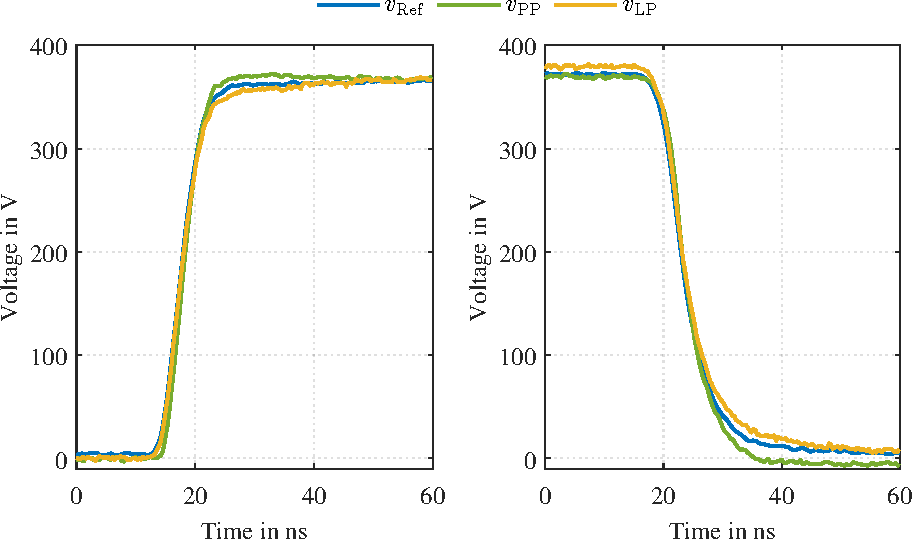
\includegraphics[scale=1]{figures/4_VoltageProbe/MS_PulsGen_TD.pdf}
	\caption{Large-signal verification time-domain of the low-pass using a \SI{50}{\ohm} pulse generator~\cite{kragl_active_2025}. The reference is acquired both via a conventional direct measurement and through a commercial \SI{180}{MHz}--\SI{340}{MHz} passive band-pass filter.}\label{fig:MS_PulsGen_TD}
\end{figure}

Datasheet for LP op states: 800MHz at 200mV, 250MHz at 2V and 140MHz at 4V. Plus BUF 3.1Ghz at 100mVpp, 1.6 at 2Vpp ...



\begin{figure}[ht]
	\centering
	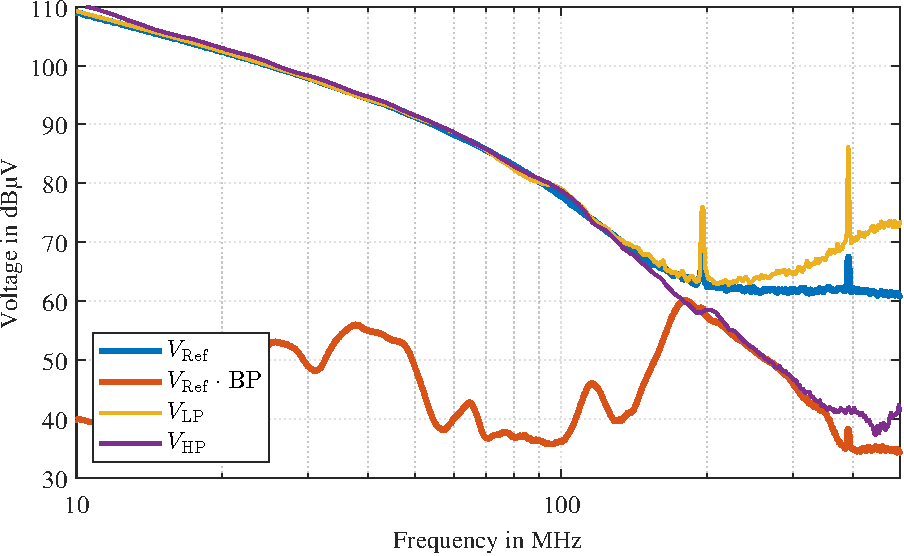
\includegraphics[scale=1]{figures/4_VoltageProbe/MS_PulsGen.pdf}
	\caption{Large-signal verification of the low-pass and high-pass channels using a \SI{50}{\ohm} pulse generator~\cite{kragl_active_2025}. The reference is acquired both via a conventional direct measurement and through a commercial \SI{180}{MHz}--\SI{340}{MHz} passive band-pass filter.}\label{fig:MS_PulsGen_Meas}
\end{figure}


% \begin{figure}[ht]
% 	\centering
% 	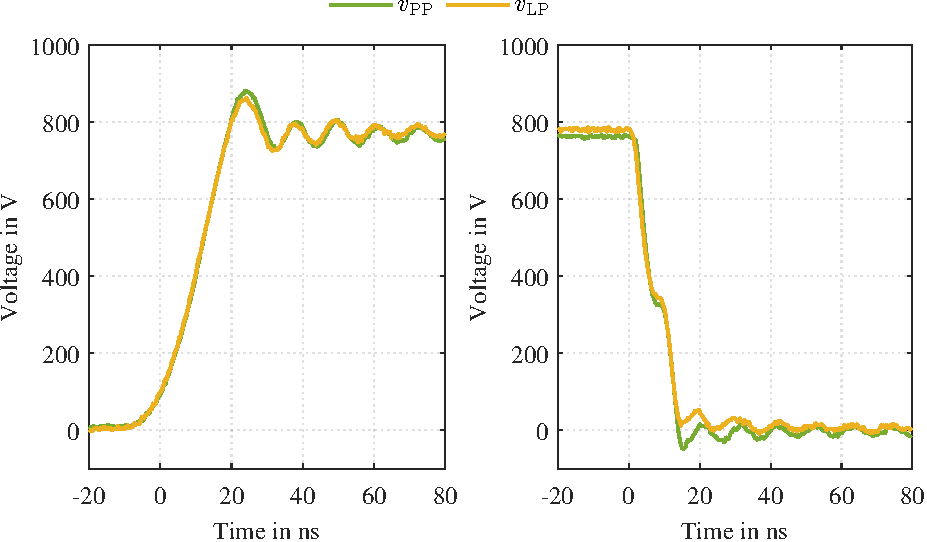
\includegraphics[scale=1]{figures/4_VoltageProbe/Voltage_DPT_EMEvsPP_TD.pdf}
% 	\caption{Time-domain measurement results of PMTX05, at 800V, 30A room temperature, cross validation of passive probe and low-pass measurement to crosscheck inductive and capacitive coupling effects.}\label{fig:Voltage_DPT_EMEvsPP_TD}
% \end{figure}


\subsection{Parasitic Couplings \& CM error}

\begin{figure}[ht]
	\centering
	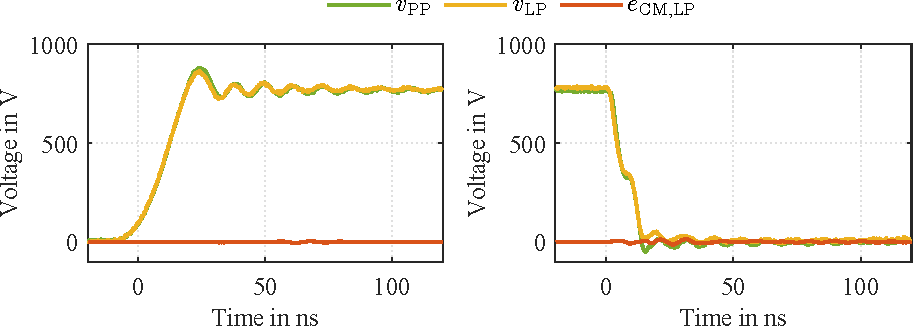
\includegraphics[scale=1]{figures/4_VoltageProbe/Voltage_DPT_LPvsPP_weCM_TD.pdf}
	\caption{Time-domain measurement results of PMTX05, at 800V, 30A room temperature, cross validation of passive probe and low-pass measurement to crosscheck inductive and capacitive coupling effects.}\label{fig:Voltage_DPT_LPvsPP_weCM_TD}
\end{figure}

\begin{figure}[ht]
	\centering
	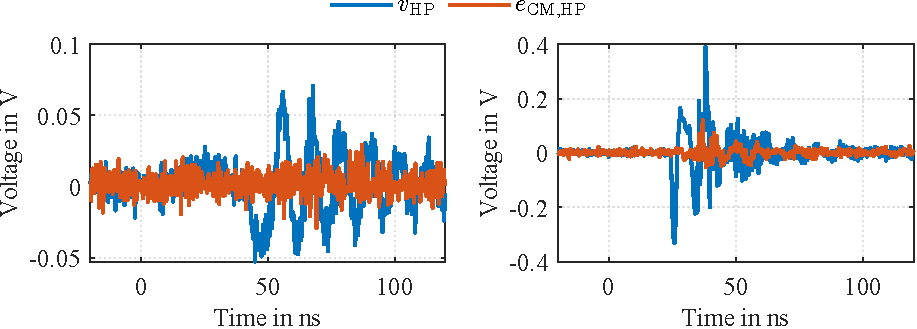
\includegraphics[scale=1]{figures/4_VoltageProbe/Voltage_DPT_HPvsPP_weCM_TD.pdf}
	\caption{Time-domain measurement results of PMTX05, at 800V, 30A room temperature, cross validation of passive probe and high-pass measurement to crosscheck inductive and capacitive coupling effects.}\label{fig:Voltage_DPT_HPvsPP_weCM_TD}
\end{figure}


The verification results demonstrate close agreement between the reference and the probe measurement for both the low-pass and high-pass channels in their respective frequency ranges.
The high-pass channel exhibits a maximum deviation of \SI{1.3}{dB} at \SI{200}{MHz}.
Above \SI{340}{MHz}, verification is no longer possible, as the commercial band-pass filter rolls off in this region.
No commercially available band-pass filter covers the \SIrange{300}{400}{MHz} frequency region, preventing independent verification in this range.

However, above \SI{340}{MHz}, the spectrum exhibits a plateau rather than the expected continuous decrease, indicating a measurement artifact that may increase the error beyond \SI{1.3}{dB} at higher frequencies.

Overall, the measurements demonstrate high repeatability, and the \SI{1.3}{dB} maximum deviation is considered sufficiently small for the intended analysis.
For the following analysis, the spectra are shown up to \SI{500}{MHz}, but the reader should be aware that the probe is only fully verified up to \SI{340}{MHz}.
Hence, results between \SI{340}{MHz} and \SI{500}{MHz} should be interpreted comparatively rather than as absolute calibrated values.
